\textbf{Photometric study of single-shot energy-dispersive X-ray
diffraction at a laser plasma facility}

O.R. Hoidn and G.T. Seidler\textsuperscript{(*)}

Physics Department

University of Washington

Seattle WA 98195-1560

\textbf{Abstract}

The low repetition rates and possible shot-to-shot variations in
laser-plasma studies place a high value on single-shot diagnostics. For
example, white-beam scattering methods based on broadband backlighter
x-ray sources are used to determine changes in the structure of
laser-shocked crystalline materials by the evolution of coincidences of
reciprocal lattice vectors and kinematically-allowed momentum transfers.
Here, we demonstrate that white-beam techniques can be extended to
strongly-disordered dense plasma and warm dense matter (WDM) systems
where reciprocal space is only weakly structured and spectroscopic
detection is consequently needed to determine the static structure
factor and thus the ion-ion radial distribution function. Specifically,
we report a photometric study of energy-dispersive diffraction (ED-XRD)
for structural measurement of high energy density systems at large-scale
laser facilities such as OMEGA and the National Ignition Facility. We
find that structural information can be obtained in single-shot ED-XRD
experiments using established backlighter and spectrometer technologies.

(*) Corresponding author:
\href{mailto:seidler@uw.edu}{\emph{seidler@uw.edu}}

Draft: 9/2/2013

\subsection{I Introduction}\label{i-introduction}

In addition to their centrality for inertial confinement fusion
studies,\hyperref[j.-d.-lindl-p.-amendt-r.-l.-berger-s.-g.-glendinning-s.-h.-glenzer-s.-w.-haan-r.-l.-kauffman-o.-l.-landen-and-l.-j.-suter-physics-of-plasmas-11-339-2004.]{\textsuperscript{1}}\textsuperscript{,}
\hyperref[e.-i.-moses-nuclear-fusion-49-104022-2009.]{\textsuperscript{2}}
laser-shock experiments play a growing role at the interface between
plasma physics and condensed matter physics, geosciences, and laboratory
astrophysics.\hyperref[f.-langenhorst-m.-boustie-a.-migault-and-j.-p.-romain-earth-and-planetary-science-letters-173-333-1999.]{\textsuperscript{3-14}}
However, for experiments reaching the highest energy density states the
technical challenges extend beyond the creation of such states: the low
repetition rates, limited facility access, and significant shot-to-shot
variations each place a special emphasis on single-shot x-ray
diagnostics of the structural and electronic properties of the
compressed, heated
target.\hyperref[b.-k.-f.-young-et-al.-review-of-scientific-instruments-69-4049-1998.]{\textsuperscript{15-24}}
An important case-in-point is provided by the determination of the
ion-ion radial distribution function,
\(g_{\text{ii}}\left( \overrightarrow{r} \right)\), or equivalently the
static structure factor \(S(\overrightarrow{k})\). Knowledge of
\(g_{\text{ii}}\left( \overrightarrow{r} \right)\) fulfills an
interesting variety of roles. First, it is necessary, if only at the
level of mean density and average ionization state, for investigation of
any equations of state (EOS) and of molecular dynamics simulations or
other structural calculations performed in support of EOS calculations.
Second, it is also a critical input parameter to any fine treatment of
electronic structure. The electronic structure of dense crystalline
systems and plasmas, in turn, is a quantity of fundamental interest but
also of a certain pragmatic interest: some sufficient knowledge of
electronic structure is needed for reliable determination of the target
temperature and ionization state in dense plasma and warm dense matter
(WDM) experiments
\hyperref[s.-h.-glenzer-and-r.-redmer-reviews-of-modern-physics-81-1625-2009.]{\textsuperscript{25}}\textsuperscript{,}
\hyperref[g.-gregori-et-al.-physics-of-plasmas-11-2754-2004.]{\textsuperscript{26}}\hyperref[s.-h.-glenzer-and-r.-redmer-reviews-of-modern-physics-81-1625-2009.]{},
and this capability is in turn needed for campaigns to experimentally
measure the EOS in the WDM regime
\hyperref[h.-j.-lee-et-al.-physical-review-letters-102-115001-2009.]{\textsuperscript{27-29}}.

For targets that retain substantial medium- or long-range order upon
shock compression, broadband backlighter x-ray sources enable white-beam
angle-dispersive x-ray diffraction (AD-XRD) in which substantial
structural detail can be inferred from Kossel rings
\hyperref[v.-lider-crystallography-reports-56-169-2011.]{\textsuperscript{30}}
and other fine scattering patterns dictated by the coincidence of
reciprocal lattice vectors and kinematically-allowed momentum transfers
\hyperref[m.-suggit-g.-kimminau-j.-hawreliak-b.-remington-n.-park-and-j.-wark-review-of-scientific-instruments-81-083902-2010.]{\textsuperscript{31}}\textsuperscript{,}
\hyperref[m.-j.-suggit-et-al.-nature-communications-3-1224-2012.]{\textsuperscript{32}}.
However, white-beam AD-XRD is only applicable to systems that are
substantially single crystalline: any statistically isotropic system,
whether a polycrystalline fine-powder sample or a dense, partially
ionized plasma, when illuminated by a broad-band source will show an
angularly-featureless signal when observed on, \emph{e.g}., an image
plate. For high atomic number (Z) systems, single-shot white-beam
extended x-ray absorption fine structure (EXAFS) has seen some
applications
\hyperref[b.-yaakobi-t.-r.-boehly-d.-d.-meyerhofer-t.-j.-b.-collins-b.-a.-remington-p.-g.-allen-s.-m.-pollaine-h.-e.-lorenzana-and-j.-h.-eggert-physical-review-letters-95-075501-2005.]{\textsuperscript{33}};
the situation has proven more challenging for lower-Z WDM and dense
plasmas, as a result of the mutually-exclusive target thickness
requirements of the x-ray measurement (soft x-ray penetration lengths of
order 1 micron or less) and laser ablation (necessary thicknesses of
tens of microns)
\hyperref[j.-l.-bourgade-et-al.-review-of-scientific-instruments-75-4204-2004.]{\textsuperscript{34}}.
Consequently, the first determination of
\(g_{\text{ii}}\left( r \right)\) for disordered, dense lower-Z plasma
systems
\hyperref[t.-ma-et-al.-physical-review-letters-110-065001-2013.]{\textsuperscript{35}}
instead used multi-shot, quasi-monochromatic AD-XRD, \emph{i.e.},
`traditional' XRD.

Here, we investigate whether single-shot, white-beam XRD can be
performed on \emph{strongly disordered}, laser-shocked solids and WDM
using spectral information at the detector location to parameterize the
momentum transfer of the quasielastic scattering event, \emph{i.e.,} we
consider purely energy-dispersive x-ray diffraction (ED-XRD). Some
context is needed to fully define this term and to distinguish it from
XRD methods already in use in the laser-plasma community. The
differential scattering cross section per atom for coherent scattering
of x rays (ordinary diffraction of incoherent incident photons) from an
isotropically disordered, elemental material such as a powder sample,
liquid, or dense laser-shock heated plasma of a single atomic species is

\(\frac{d\sigma_{\text{coh}}}{\text{dΩ}}\left( k \right) = \sigma_{t}S\left( k \right){f\left( k \right)}^{2}\)
(1)

where \(\sigma_{t}\) is the Thomson cross section, \(S(k)\) is the
directionally-averaged structure factor and \(f\left( k \right)\) is the
spherically averaged atomic form factor. The structure factor \(S(k)\)
is simply related by a sine transform to
\(g_{\text{ii}}\left( r \right)\),

\(S\left( k \right) = 1 + (4\ \pi\ \rho/k)\ \int_{0}^{\infty}{dr\ r\ \lbrack\ g_{\text{ii}}\left( r \right) - 1\rbrack}\ \sin{(kr})\).
(2)

These well\emph{-}known expressions establish the close connection
between XRD and \(g_{\text{ii}}\left( r \right)\) while also
demonstrating the need to measure the differential scattering
cross-section (and hence \(S(k)\)) at many different momentum transfers
if any significant constraint on the form of
\(g_{\text{ii}}\left( r \right)\) is to be obtained.

The \(k\)-dependence of \(d\sigma_{\text{coh}}/d\Omega\) can in
principle be measured with any suitable combinations of scattering angle
\(2\theta\) and photon energies spanning the needed momentum transfers:
\(k\) is chosen by the combined effect of these two
experimentally-selectable parameters,
\(k = \operatorname{(2E/c)sin}{2\theta}\). In practice, however, XRD is
measured in only two modes: angle-resolved XRD (henceforth `AR-XRD') and
energy-dispersive XRD (henceforth `ED-XRD'). Their distinction is best
introduced kinematically. As illustrated in Fig. 1, any measurement of
\(S(k)\) must follow a curve in \(E\)-\(2\theta\) space which crosses
many of the shown contours of constant \emph{k.} The parameter space
probed by a typical AR-XRD experiment using \textasciitilde{}8 keV
monochromatic incident photons is represented by the vertical curve in
the figure. Experimentally, the necessary apparatus will include a
monochromatic source and either an angle-scanning detector or a position
sensitive detector (PSD), which we show schematically in Fig. 2 (a) and
(b). On the other hand, a typical ED-XRD experiment instead resides on
the horizontal curve in Fig. 1, \emph{i.e.}, at a fixed scattering angle
of 135 degrees but requiring both a broad incident source spectrum and
an energy-resolving detector. An experimental schematic for ED-XRD is
presented in Fig. 2(c). We note that ED-XRD has a long history in
laboratory and synchrotron XRD studies, and plays an important role in
high-pressure diamond anvil cell research where the limited angular
access to the sample space substantially complicates
AD-XRD.\hyperref[y.-feng-m.-somayazulu-r.-jaramillo-t.-rosenbaum-e.-isaacs-j.-hu-and-h.-k.-mao-review-of-scientific-instruments-76-063913-2005.]{\textsuperscript{36-40}}
There is then an obvious commonality with experiments at large-scale
laser facilities; angular access at such facilities is strongly
constrained by the beam paths of the laser light itself.

AD-XRD from laser-shock compressed, disordered Al has recently been
reported by Ma, \emph{et
al.},\hyperref[t.-ma-et-al.-physical-review-letters-110-065001-2013.]{\textsuperscript{35}}
and this first such study illustrates both the scientific benefits and
technical drawbacks of AD-XRD for large-scale laser facilities.
Specifically, concerning the latter, a few high-resolution spectrometers
must be moved between different scattering angles for different shots so
as to obtain a complete characterization of \(S(k)\) by pooling the
results of many shots after suitable normalization or other
characterization of shot-to-shot variations in the source or target.
While the study of Ma, \emph{et
al.},\hyperref[t.-ma-et-al.-physical-review-letters-110-065001-2013.]{\textsuperscript{35}}
has overcome these challenges and provides an interesting comparison of
experiment to modern theoretical treatments of the structure of dense
plasmas, it is still important to note that the use of a multi-shot
technique has, at a minimum, decreased the range of phase space that can
be studied subject to the strong constraints that exist on facility
access. A single-shot alternative could therefore have high scientific
impact and is likely the only way that \(S(k)\) will be measured on
disordered dense plasmas at the National Ignition Facility, where the
number of shots per scientific study is especially limited.

Consequently, with the above context established, we report here a
photometric analysis of ED-XRD for laser-shock experiments illuminated
by broad-band backlighter sources. This analysis makes use of known
results for the spectrum of a broad-band backlighter, representative
experimental results for \(S(k)\) for disordered systems, and
representative, established technical characteristics of
spectrally-resolving detectors available at large-scale laser
facilities. We find significant benefits to ED-XRD for disordered
systems, including single-shot determination of \(S(k)\), and we propose
that ED-XRD should become a standard diagnostic at large-scale
facilities such as OMEGA and the National Ignition Facility

We continue as follows. In section 2 we describe the methods used in the
photometric analysis, including the reference target, modeled
experimental geometry, and any assumptions about detector or
spectrometer performance. In section 3 we present and discuss our
results for ED-XRD using each of two different experimental
configurations. These are, first, an x-ray CCD detector operating in
single-photon mode as an energy-resolving solid-state detector and,
second, a wavelength-dispersive spectrometer using a highly-oriented
pyrolytic graphite (HOPG) mosaic crystal as the diffractive element. The
CCD configuration is viable, but has some drawbacks associated with
saturation and double-counting that require special care. We find that
the HOPG-based spectrometer quite easily resolves the energy spectrum of
the diffraction with excellent counting statistics for a broad-band
backlighter that has been fielded at OMEGA, with the caveat that a
single HOPG crystal analyzer covers a narrower energy range, and hence a
more restricted \(k\)-range, than a CCD detector. Finally, in section IV
we conclude.

\subsection{II Methods}\label{ii-methods}

\textbf{II.A. Source and target}

One readily available broadband source in laser shock experiments is the
thermal spectrum from a laser-imploded polymer shell, usually filled
with H\textsubscript{2}-D\textsubscript{2} gas
\hyperref[b.-r.-maddox-et-al.-physics-of-plasmas-18-056709-2011.]{\textsuperscript{41}}\textsuperscript{,}
\hyperref[b.-yaakobi-f.-j.-marshall-t.-r.-boehly-r.-p.-j.-town-and-d.-d.-meyerhofer-journal-of-the-optical-society-of-america-b-optical-physics-20-238-2003.]{\textsuperscript{42}}.
In Fig. 3 we show a typical spectrum collected at OMEGA
\hyperref[b.-yaakobi-2012-private-communication.]{\textsuperscript{43}}.
Because of the spectrum's supra-exponential decay, an ED-XRD experiment
with this source is preferentially conducted at low energy, between 2
and 6 keV, as shown in the ED-XRD curve at a scattering angle of 135
degrees in Fig. 1. Also shown in Fig. 3 is the spectrum for a typical
narrow band backlighter source at OMEGA, where these sources have seen
extensive use in x-ray scattering studies, both elastic (XRD)
\hyperref[t.-ma-et-al.-physical-review-letters-110-065001-2013.]{\textsuperscript{35}}
and inelastic (usually called `x-ray Thomson scattering')
\hyperref[s.-h.-glenzer-and-r.-redmer-reviews-of-modern-physics-81-1625-2009.]{\textsuperscript{25}}.
The narrow-band spectrum is obtained by scaling the spectrum of a Cu
\emph{K\textsubscript{α}} target driven by a 10 J, 10 ps laser pulse at
the MTW laser facility to a 2.5 kJ, 10 ps laser pulse at OMEGA, using a
typical \emph{K\textsubscript{α}} photon yield of 4 ×
10\textsuperscript{10} photons per J of laser energy
\hyperref[p.-m.-nilson-2012-private-communication.]{\textsuperscript{44}}\textsuperscript{,}
\hyperref[k.-u.-akli-et-al.-physics-of-plasmas-14-023102-2007.]{\textsuperscript{45}}.

We consider two target systems where experimental \(S(k)\) are
available: liquid boron at ambient pressure and shock-compressed
aluminum. For liquid boron we use the experimental results of Krishnan
\emph{et al.}
\hyperref[s.-krishnan-s.-ansell-j.-j.-felten-k.-j.-volin-and-d.-l.-price-physical-review-letters-81-586-1998.]{\textsuperscript{46}}\textsuperscript{,}
\hyperref[s.-krishnan-and-d.-l.-price-journal-of-physics-condensed-matter-12-r145-2000.]{\textsuperscript{47}},
the data for which were taken at a synchrotron light source using
hydrodynamically-levitated boron heated to 2400K by continuous
illumination from infrared lasers. While this is not a WDM system
\emph{per se}, it is a reasonable surrogate. As shown in Fig. 4 (a),
note the presence of a few broad peaks in \(S(k)\), representative of a
system with only limited, short-range information in
\(g_{\text{ii}}\left( r \right)\). For clarity in our photometric
analysis, we will use a smoothed \(S(k)\) where the sharp (nonphysical)
noise in the experimental \(S(k)\) has been filtered. On the other hand,
\(S(k)\) for shock-compressed aluminum (\(n_{e}\)= 5.4 ×
10\textsuperscript{23} cm\textsuperscript{-3}; \(T_{e}\)= 10 eV) is
based on results from Ma \emph{et
al.}\hyperref[t.-ma-et-al.-physical-review-letters-110-065001-2013.]{\textsuperscript{35}},
who have recently reported the first AD-XRD measurement of a
shock-compressed, disordered WDM system. \(S(k)\) was recovered from Ma
\emph{et al.}'s theoretical calculation of an elastic scattering profile
for triply-ionized shock-compressed aluminum, to which they fit their
data. We note that only an approximate atomic form factor, that of
ambient aluminum, was used to calculate \(S(k)\) from the scattering
profile; however, the resulting error in \(S(k)\) is expected to be
negligible above \(k = 3A^{- 1}\), and hence does not affect the
location of any coordination peaks. As shown in Fig. 4 (b), note again
that the presence of only short-range order in the target results in a
simple form for \(S(k)\). In this case, the information content is
largely limited to the location and intensity of the obvious first
coordination peak.

\textbf{II.B. Photon-electron interactions and numerical modeling }

For the targets considered here, the experiment is conducted in an
energy region far above any atomic fluorescence from the targets and
also far above any soft x-ray blackbody radiation from the surface or
bulk of the target, each of which is easily attenuated in practice with
a thin plastic or Be shield. Consequently, we need only consider the
coherent and incoherent scattering of the x-rays as direct contributors
to the measured scattering signal; the photoelectric interaction appears
only in its contribution to absorption coefficient in the energy range
of interest. Note that by coherent here we refer to the quasielastic
scattering process itself, \emph{i.e.} ``ordinary'' diffraction, with no
expectation of coherence of the incident beam (such as is used in
diffraction experiments at XFEL facilities).

Given a backlighter source with fluence
\(I_{\text{source}}\left( E \right)\) (units of photons/eV, integrated
over 4π steradian) at a distance \(d_{\text{source}}\) from the target,
the areal flux incident in the target is
\(I_{\text{incident}}\left( E \right) = I_{\text{source}}\left( E \right)/4\pi d_{\text{source}}^{2}\).
The contribution of coherent scattering to the measured energy spectrum
at a scattering angle \(2\theta\) is then

\(I_{\text{coh}}\left( E,2\theta \right) = I_{\text{incident}}\left( E \right)\ \frac{d\sigma_{\text{coh}}}{\text{dΩ}}\left( k \right)\text{\ d}\Omega_{\det}\ \eta_{\det}\left( E \right)\ \tau_{\text{coh}}\left( E,2\theta \right)\),
(3)

where \(k\) is implicitly determined by \(E\) and \(2\theta\) ,
\(d\Omega_{\det}\) is the solid angle subtended by the detector,
\(\eta_{\det}\left( E \right)\) is the net efficiency of detection of
photons of energy \(E\) that arrive in \(d\Omega_{\det}\), and
\(\tau_{\text{coh}}\left( E,2\theta \right)\) includes the necessary
corrections to the measured XRD due to the target's geometry and
energy-dependent absorption coefficient
\hyperref[j.-l.-bourgade-et-al.-review-of-scientific-instruments-75-4204-2004.]{\textsuperscript{34}}.
When operating near to a backscattering geometry, for example,
\(\tau_{\text{sample}}\left( E,2\theta \right)\ \ \sim\ \rho\ A(1 - \ e^{- 2\ \mu\left( E \right)d})/2\ \mu(E)\ \)where
\(\rho\) is atomic (number) density, \(A\) is the cross-sectional area
of the portion of the backlighter beam that illuminates the target
region of interest, \(d\) is the target thickness, and
\(\mu\left( E \right)\) is the x-ray absorption coefficient. For present
purposes, \(d\sigma_{\text{coh}}/d\Omega\) includes all elastic and
quasielastic scattering; it integrates over all ion-ion correlation
dynamics
\hyperref[g.-gregori-and-d.-o.-gericke-physics-of-plasmas-16-056306-2009.]{\textsuperscript{48}}.

The incoherent contribution to the measured signal is somewhat more
complex to model. The microscopic physics of the incoherent scattering
processes, wherein one must address both momentum transfer (\(k\)) and
energy transfer (\(\text{ℏω}\)), results in the need for a double
differential cross-section
\(d^{2}\sigma_{\text{incoh}}\frac{\left( k,\omega \right)}{\text{dωd}}\Omega\).
The detected intensity from incoherent scattering is then

\(I_{\text{incoh}}\left( E,\ 2\theta \right) = d\Omega_{\det}N_{\text{atoms}}\ \frac{d\sigma_{t}}{d\Omega}\int_{0}^{\infty}{dE'I_{\text{incident}}\left( E' \right)}\ S_{\text{incoh}}\left( k,\ \omega \right)\tau_{\text{incoh}}\left( E^{'},E,2\theta \right)\)
(4),

where \(N_{\text{atoms}}\) is the number of atoms in the target, \(k\)
is again implicitly determined by \(E\), \(E'\)\emph{,} and \(2\theta\)
and \(\tau_{\text{incoh}}\left( E^{'},E,2\theta \right)\) includes the
influence of attenuation for an incident photon of energy \(E'\) that
scatters through an angle \(2\theta\) and departs the incoherent
interaction with energy \(E\). In the first Born approximation,
\(d^{2}\sigma_{\text{incoh}}/d\omega d\Omega = (d\sigma_{t}/d\Omega)\ S_{\text{incoh}}\left( k,\ \omega \right),\)
where \(d\sigma_{t}/d\Omega\) is the Thomson differential scattering
cross section and \(S_{\text{incoh}}\left( k,\ \omega \right)\) is the
inelastic component of the dynamic structure factor. In the
independent-electron approximation
\hyperref[j.-chihara-journal-of-physics-condensed-matter-12-231-2000.]{\textsuperscript{49}}\textsuperscript{,}
\hyperref[w.-schuelke-electron-dynamics-by-inelastic-x-ray-scattering-oxford-university-press-new-york-2007.]{\textsuperscript{50}},
\(S_{\text{incoh}}\left( k,\ \omega \right)\) may be expressed as a sum
over electrons and matrix elements between the initial and final states
of the system:

\(S_{\text{incoh}}\left( k,\ \omega \right) = \ \sum_{j}^{}{\sum_{f \neq i}^{}{\left| \left\langle {i|e}^{\text{i\ }\mathbf{q \bullet}\mathbf{r}_{\mathbf{j}}}|f \right\rangle \right|^{2}\delta(E_{f} - \ E_{i} - \ \omega)}}\).
(5)

At sufficiently high
\(k\),\(\ S_{\text{incoh}}\left( k,\ \omega \right)\) is peaked at the
Compton shift \(\Delta E = \ ^{2}k^{2}/2\ m\). In the high\emph{-}\(k\)
(non-collective) scattering regime the total inelastic portion of the
dynamic structure factor is constructed using equation (5) evaluated as
a sum over individual valence and core electrons. In our modeling
procedure this consists of truncated valence and core Compton profiles
generated in the impulse approximation
\hyperref[w.-schuelke-electron-dynamics-by-inelastic-x-ray-scattering-oxford-university-press-new-york-2007.]{\textsuperscript{50}}\textsuperscript{,}
\hyperref[p.-eisenberger-and-p.-m.-platzman-physical-review-a-2-415-1970.]{\textsuperscript{51}}
where \(S_{\text{incoh}}\left( k,\ \omega \right)\) depends only on the
ground state electronic density and kinematics of the scattering
process. The first moment of
\(\ S_{\text{incoh}}\left( k,\omega \right)\) was normalized after
truncation according to the Bethe \emph{f}-sum rule
\hyperref[b.-a.-mattern-g.-t.-seidler-j.-j.-kas-j.-i.-pacold-and-j.-j.-rehr-physical-review-b-85-115135-2012.]{\textsuperscript{52}}.
For boron our approximation yields incoherent scattering cross sections
which exceed experimental values by up to 30 percent, making our
approximate treatment of the incoherent background conservative. In the
relevant range of momentum transfers the Compton shift is sufficiently
small that we substitute \(\tau_{\text{coh}}\left( E,2\theta \right)\)
for \(\tau_{\text{incoh}}\left( E,\ E',2\theta \right)\) without
introducing appreciable systematic error, allowing \(\tau\) to be
factored out of the integrand in equation (4). Similarly, the FWHM of
\(\ S_{\text{incoh}}\left( k,\ \omega \right)\) (which, in the impulse
approximation, is directly related to the width of the momentum
distribution of the electronic ground state) is small compared to our
required energy resolution, such that we can define a Compton-shifted
energy variable \(E^{*} = E + \ \Delta E\) and re-express (4) in
approximate form:

\(I_{\text{incoh}}\left( E,2\theta \right) = d\Omega_{\det}N_{\text{atoms}}\text{\ \ }\frac{d\sigma_{t}}{d\Omega}\ \tau_{\text{coh}}\left( E,2\theta \right)\ I_{\text{incident}}\left( E^{*} \right)\int_{0}^{\infty}{dE'}\text{\ \ }S_{\text{incoh}}\left( k,\ \omega \right)\).
(6)

The total scattered intensity, in units of photons/sr, is then

\subparagraph{\texorpdfstring{\(\mathbf{I}_{\mathbf{\text{total}}}\left( \mathbf{E} \right)\mathbf{= \ }{\mathbf{d}\mathbf{\Omega}_{\mathbf{\det}}\mathbf{\text{\ N}}}_{\mathbf{\text{atoms}}}\mathbf{\ }\mathbf{\tau}\left( \mathbf{E,\ 2}\mathbf{\theta} \right)\mathbf{\ }\frac{\mathbf{d}\mathbf{\sigma}_{\mathbf{t}}}{\mathbf{d}\mathbf{\Omega}}\mathbf{\ }\left\lbrack \mathbf{I}_{\mathbf{\text{incident}}}\left( \mathbf{E} \right)\mathbf{\ }{\mathbf{f}\left( \mathbf{k} \right)}^{\mathbf{2}}\mathbf{S}\left( \mathbf{k} \right)\mathbf{+ \ }\mathbf{\ }\mathbf{I}_{\mathbf{\text{incident}}}\left( \mathbf{E}^{\mathbf{*}} \right)\int_{\mathbf{0}}^{\mathbf{\infty}}{\mathbf{d}\mathbf{E}^{\mathbf{'}}}\mathbf{\text{\ \ }}\mathbf{S}_{\mathbf{\text{incoh}}}\left( \mathbf{k,\ \omega} \right) \right\rbrack\mathbf{\text{.\ }}\)(7)}{\textbackslash{}mathbf\{I\}\_\{\textbackslash{}mathbf\{\textbackslash{}text\{total\}\}\}\textbackslash{}left( \textbackslash{}mathbf\{E\} \textbackslash{}right)\textbackslash{}mathbf\{= \textbackslash{} \}\{\textbackslash{}mathbf\{d\}\textbackslash{}mathbf\{\textbackslash{}Omega\}\_\{\textbackslash{}mathbf\{\textbackslash{}det\}\}\textbackslash{}mathbf\{\textbackslash{}text\{\textbackslash{} N\}\}\}\_\{\textbackslash{}mathbf\{\textbackslash{}text\{atoms\}\}\}\textbackslash{}mathbf\{\textbackslash{} \}\textbackslash{}mathbf\{\textbackslash{}tau\}\textbackslash{}left( \textbackslash{}mathbf\{E,\textbackslash{} 2\}\textbackslash{}mathbf\{\textbackslash{}theta\} \textbackslash{}right)\textbackslash{}mathbf\{\textbackslash{} \}\textbackslash{}frac\{\textbackslash{}mathbf\{d\}\textbackslash{}mathbf\{\textbackslash{}sigma\}\_\{\textbackslash{}mathbf\{t\}\}\}\{\textbackslash{}mathbf\{d\}\textbackslash{}mathbf\{\textbackslash{}Omega\}\}\textbackslash{}mathbf\{\textbackslash{} \}\textbackslash{}left\textbackslash{}lbrack \textbackslash{}mathbf\{I\}\_\{\textbackslash{}mathbf\{\textbackslash{}text\{incident\}\}\}\textbackslash{}left( \textbackslash{}mathbf\{E\} \textbackslash{}right)\textbackslash{}mathbf\{\textbackslash{} \}\{\textbackslash{}mathbf\{f\}\textbackslash{}left( \textbackslash{}mathbf\{k\} \textbackslash{}right)\}\^{}\{\textbackslash{}mathbf\{2\}\}\textbackslash{}mathbf\{S\}\textbackslash{}left( \textbackslash{}mathbf\{k\} \textbackslash{}right)\textbackslash{}mathbf\{+ \textbackslash{} \}\textbackslash{}mathbf\{\textbackslash{} \}\textbackslash{}mathbf\{I\}\_\{\textbackslash{}mathbf\{\textbackslash{}text\{incident\}\}\}\textbackslash{}left( \textbackslash{}mathbf\{E\}\^{}\{\textbackslash{}mathbf\{*\}\} \textbackslash{}right)\textbackslash{}int\_\{\textbackslash{}mathbf\{0\}\}\^{}\{\textbackslash{}mathbf\{\textbackslash{}infty\}\}\{\textbackslash{}mathbf\{d\}\textbackslash{}mathbf\{E\}\^{}\{\textbackslash{}mathbf\{'\}\}\}\textbackslash{}mathbf\{\textbackslash{}text\{\textbackslash{} \textbackslash{} \}\}\textbackslash{}mathbf\{S\}\_\{\textbackslash{}mathbf\{\textbackslash{}text\{incoh\}\}\}\textbackslash{}left( \textbackslash{}mathbf\{k,\textbackslash{} \textbackslash{}omega\} \textbackslash{}right) \textbackslash{}right\textbackslash{}rbrack\textbackslash{}mathbf\{\textbackslash{}text\{.\textbackslash{} \}\}(7)}}\label{mathbfiux5fmathbftexttotalleft-mathbfe-rightmathbf-mathbfdmathbfomegaux5fmathbfdetmathbftext-nux5fmathbftextatomsmathbf-mathbftauleft-mathbfe-2mathbftheta-rightmathbf-fracmathbfdmathbfsigmaux5fmathbftmathbfdmathbfomegamathbf-leftlbrack-mathbfiux5fmathbftextincidentleft-mathbfe-rightmathbf-mathbffleft-mathbfk-rightmathbf2mathbfsleft-mathbfk-rightmathbf-mathbf-mathbfiux5fmathbftextincidentleft-mathbfemathbf-rightintux5fmathbf0mathbfinftymathbfdmathbfemathbfmathbftext-mathbfsux5fmathbftextincohleft-mathbfk-omega-right-rightrbrackmathbftext.-7}

Note that
\(\int_{0}^{\infty}{dE'}\ S_{\text{incoh}}\left( k,\ \omega \right) = N\)
(the atomic number of the scattering species) in the high\emph{-}\(k\)
limit of the impulse
approximation\hyperref[p.-eisenberger-and-p.-m.-platzman-physical-review-a-2-415-1970.]{\textsuperscript{51}}
and takes on smaller values at lower momentum transfers; by comparison,
\({f(0)}^{2} = N^{2}\), and \(S(k)\) is of order unity. Therefore the
first (coherent) term in \(I_{\text{total}}\left( E \right)\) dominates
for heavier elements or for sufficiently small momentum transfers. In
Fig. 5 (a) and (b) we compare \({f(k)}^{2}\) to the incoherent
background scattering for the above-described model. These results lead
us to expect that the background in an ED-XRD experiment will not
substantially limit the ability to observe the desired coherent
scattering.

\textbf{II.C. Spectrometers for detection of ED-XRD}

We now consider two different detection options. As shown in the
schematic of Fig. 2, one or both of an x-ray CCD and a HOPG-based
spectrometer may be used as energy-sensitive detectors. Simulated
spectra for both follow in section III. Throughout the remainder of the
paper the following experimental parameters are used:
\(d_{\text{source}}\) = 1 cm; target dimensions (for both B and Al):
0.25 mm × 0.25 mm × 0.1 mm; scattering angle \(2\theta\) = 135 degrees.
These choices will be motivated below.

The modeled CCD has a 2-dimensional square grid of 2200 x 2200 pixels,
with a pixel edge length of 13.5 microns. A quantum efficiency of 1 is
assumed. The optimal distance between the detector and the target is
determined by the competing demands of high signal collection and high
rejection of two-photon events on single pixels. We find it reasonable
to balance these demands by selecting a single photon-hit regime with an
expectation value \(p\) of 0.1 photon hits per pixel. At a given
scattering angle and in the absence of addition of any special absorbers
between the target and the CCD other than a Be filter for low-energy
photon rejection, \(p\) is determined by the working distance of the CCD
and the scattered intensity off the target. The working distance is not
a highly-constrained parameter; it must merely be sufficiently large
that backgrounds from the high neutron flux and other stray radiations
are likely to be substantially suppressed. An upper bound on target
intensity arises from signal broadening due to the finite angular size
subtended by the target relative to the backlighter. We require this
geometrical broadening in momentum transfer, \(\text{Δk}\)\emph{,} to
satisfy \(\Delta k/k\ \  < \ 0.05\), such that it is sufficiently small
compared to the intrinsic scale of structure in \(S(k)\). We label the
angle subtended by the target \(\Delta\theta_{t}\) and express the
geometrical broadening in terms of it:
\(\Delta k/k\  = \ \cot{\text{θ\ Δ}\theta_{t}}.\) At
\(2\theta\  = \ 135\ degrees\) the maximal \(\Delta\theta_{t}\) is
approximately 0.1 radians, which corresponds to a sample length of 1 mm.

The task of presenting a modeled HOPG spectrum in a
non-configuration-specific manner is complicated by the significant
dependence of the spectrometer's energy range on several geometric
parameters. Using the labeling of Fig. 6 and, as an example, the
spectrometer geometry described by Fig. 7 (a), the differential in \(k\)
for scattering from the target is

\(dk = \ \frac{\text{δk}}{\text{δE}}\ dE + \ \frac{\text{δk}}{\delta(2\theta)}\ d(2\theta) = \ \frac{E}{\text{ℏc}}\left( \sin{(\theta)\ \cot{\theta_{B}\  - \ \cos{(\theta)}}}\  \right)\text{dθ}_{B}\).
(9)

As a crystal of length \(l\) located a distance \(F\) from the target
subtends an angle of approximately (\(l/F)\ \sin\theta_{B}\), we can
directly use (9) to calculate the range \(\text{Δk}\) covered by an
analyzer crystal as a function of \(k\)\emph{,}\(\ 2\theta,\) and the
choice of HOPG reflection. Fig. 7 illustrates this. Salient features of
\(\Delta k(k,\ 2\theta)\) are that it is asymptotically linear in \(k\)
and depends weakly on \(2\theta\ \)everywhere except at low
\(k\)\emph{.}

That said, we can choose a typical configuration for an HOPG
spectrometer and generate a detected spectrum that spans the entire
range of \(k\) with which we are concerned. Conceptually, this is done
by repeatedly rotating the crystal to different central \(\theta_{B}\)
to acquire narrow spectra in different ranges of \(k\) and then
stitching together the resulting spectra. This spectrum, which is
henceforth referred to as the ``HOPG source spectrum'', does not
represent a realistic data set, since acquiring it in a single shot
would require prohibitively many analyzer crystals, but it does serve as
a convenient compilation of the ensemble of possible experimental
configurations; the exact choice of spectrometer configuration for a
given experiment depends on some prior knowledge of the desired \(k\)
range, as we discuss below.

The modeled HOPG spectrometer is qualitatively similar to several
instruments that have previously been fielded for x-ray Thomson
scattering studies at OMEGA
\hyperref[y.-jae-hyuck-i.-jung-bin-p.-jong-bok-j.-hojeong-and-p.-g.-costas-applied-physics-letters-100-233124-2012.]{\textsuperscript{53-55}}.
For our modeled instrument, the HOPG diffractive element operates on the
002 reflection, has a mosaic spread of 0.3 degrees, is taken to be a
flat square with side length \(l\) = 12 cm, and is located at a distance
\(F\) \emph{=} 25 cm from the target. The energy-dependent integral
reflectivity of the HOPG is based on computed reflectivity curves
\hyperref[a.-k.-freund-a.-munkholm-and-s.-brennan-optics-for-high-brightness-synchrotron-radiation-beamlines-ii-2856-68-1996.]{\textsuperscript{56}}
for an HOPG crystal having a mosaic spread of 0.3 degrees. Denoting
\(r\) as the peak reflectivity and \(\omega\) as the FWHM of the
reflectivity curve, the angular integral reflectivity,
\(\Delta\theta_{B},\) is approximately \(\text{rω}\)\emph{;}
equivalently, the integral reflectivity in energy units is
\(\Delta E = E\cot{\theta_{B}\Delta\theta_{B}}\). We define \(E_{\max}\)
and \(E_{\min}\) as the maximum and minimum energies diffracted by the
crystal. For isotropically-scattered photons with a fixed energy \(E\)
between \(E_{\max}\) and \(E_{\min}\) the probability of reflection is
\(\eta\  = \ \Omega_{0}\Delta E/(4\ \pi\ \left( E_{\max} - \ E_{\min} \right))\),
where \(\Omega_{0} = ({l/F)}^{2}\ \sin\theta_{B}\) is the solid angle
subtended by the crystal relative to the source (units of sr).
Correspondingly, the detected spectrum resulting from
\(I_{\text{incident}}\) on the target is
\(I_{d}\left( E \right) = 4\pi\eta dI_{\text{incident}}\left( E \right)/d\Omega = \Delta\theta_{B}(l/F)dI_{\text{incident}}\left( E \right)/d\Omega\).
For reference, \(\Delta\theta_{B}l/F = 7 \times 10^{- 4}\) at 4 keV. It
will be seen in the next section that the resulting net collection
efficiency in a given achievable energy band is several orders of
magnitude higher than that of the CCD.

\subsection{III Results and
discussion}\label{iii-results-and-discussion}

There is good reason to believe, heuristically, that the above-described
experimental configurations for ED-XRD should determine
\(S\left( k \right)\) with adequate statistics. Numerous past x-ray
Thomson scattering experiments at laser plasma facilities have measured
the inelastic portion of \(S\left( k,\omega \right)\) using narrow pulse
backlighters for illumination
\hyperref[s.-h.-glenzer-and-r.-redmer-reviews-of-modern-physics-81-1625-2009.]{\textsuperscript{25}}\textsuperscript{,}
\hyperref[h.-j.-lee-et-al.-physical-review-letters-102-115001-2009.]{\textsuperscript{27}}\textsuperscript{,}
\hyperref[c.-fortmann-h.-j.-lee-t.-doeppner-r.-w.-falcone-a.-l.-kritcher-o.-l.-landen-and-s.-h.-glenzer-physical-review-letters-108-175006-2012.]{\textsuperscript{28}}\textsuperscript{,}
\hyperref[r.-tommasini-et-al.-review-of-scientific-instruments-79-10e901-2008.]{\textsuperscript{57-60}}.
Above 2 keV, a broad-band thermal backlighter has approximately 100
times the photon conversion efficiency of a short-pulse Cu
\emph{K\textsubscript{α}} backlighter (Fig. 3); additionally, the
elastic scattering cross section is typically larger than the Compton
cross section, as discussed in section II and shown in Fig. 5 (a) and 5
(b). Thus, ED-XRD should offer vastly higher signal intensity than
(quasi-monochromatic) x-ray Thomson scattering using a metal-foil
backlighter, and therefore better statistics.

In Fig. 8 we present \(I_{d}\left( E \right)\) defined in section II,
filtered by a 20 µm Be foil (to reject low-energy photons) for liquid
boron acquired on a CCD alongside the equivalent HOPG source spectrum.
The highlighted region of the HOPG source spectrum shows the energy
range covered by a specific configuration: a 12-cm long HOPG crystal at
distance \(F\) = 25 cm from the target, oriented such that the detected
spectrum is centered on the main correlation peak in \(S(k)\). This
crystal size results in a solid angle subtended by the crystal similar
to that in existing high-efficiency HOPG spectrometers
\hyperref[b.-yaakobi-2012-private-communication.]{\textsuperscript{43}}\textsuperscript{,}
\hyperref[a.-pak-g.-gregori-j.-knight-k.-campbell-d.-price-b.-hammel-o.-l.-landen-and-s.-h.-glenzer-review-of-scientific-instruments-75-3747-2004.]{\textsuperscript{61}}.
Figure 9 shows the CCD and HOPG spectra for shock-compressed Al in this
same format. \(S\left( k \right)\) reconstructed for B and Al is
presented in Figs. 10 and 11, respectively. In both these figures the
\(k\)-range probed by the specific spectrometer configuration is
highlighted. All reconstructed \(S\left( k \right)\) curves, including
those without background subtraction, show a well-defined correlation
peak. Note that the uncorrected curves overshoot the experimental
\(S\left( k \right)\) at large \(k\); this is a result of the
monotonically-increasing Compton background (as well as double-counts,
for the CCD). This background decreases relative to the XRD signal for
larger atomic numbers, as seen by comparison of Figs. 10 and 11. The
HOPG source spectrum exhibits excellent statistics (error bars
\textless{} 2 percent) relative to the CCD over the entire plotted
energy range. While deteriorating at high energy, the CCD spectrum also
has good statistics (error bars \textless{} 5 percent) below 4.5 keV.

The relative merits of the two detectors are dictated by particular
features of the ED-XRD configuration and the spectrum probed. Despite
the substantially better energy resolution of an HOPG spectrometer
compared to a Fano-noise limited CCD, energy resolution is a poor
criterion for comparison: at 135 degrees scattering angle, the
\(k\)-width of features in \(S(k)\) corresponds to a width in energy
greater than 500 eV, substantially larger than the resolution of both
the CCD and the HOPG spectrometer. Instead, the leading limitation on
data quality is shot noise at high \(k\) due to the sharp decay of the
source spectrum intensity with increasing energy.

The latter limitation is severe only for the CCD, (1) because of vastly
lower overall counts and especially (2) because the intense low-energy
portion of the incident spectrum is `echoed' as double-counts at higher
energy. In simulated CCD spectra the double-count contribution to the
detected spectrum outweighed the single-count contribution above 5 keV.
This double-count noise cannot be reduced by varying \(p\): in the
single photon-hit regime, the number of double-hits on single pixels
scales as \(p^{2}\); the associated Poisson noise scales as \(p\).
Single photon counts also scale as \(p\); as a result, above 5 keV
varying \(p\) has little effect on the signal-to-noise (\emph{i.e.}
single-to-double-count) ratio. It is instead highly preferable to carry
out an ED-XRD experiment in near-backscatter geometry, such that the
range of \(k\) in which \(S(k)\) has structure is probed by a
lower-energy region of the backlighter spectrum. In fact, the only means
of significantly improving data quality on a single hit CCD are (1)
using a detector with more pixels to improve statistics, and (2) moving
the detector closer to backscatter.

The two spectrometer types offer a variety of configurations adapted to
experimental situations in which different \(k\)-ranges need to be
probed. If the goal is to locate the main correlation peak in
\(S(k)\)\emph{,} a single-HOPG crystal spectrometer is a viable option
(illustrated, as mentioned above, in Figs. 10 and 11). On the other
hand, if the scientific goal requires a significantly wider \(k\)-range,
then a CCD detector in single photon counting mode, multiple HOPG
analyzer crystals, or both are necessary. Despite the CCD's relatively
poor signal to noise ratio, there is substantial motivation for
performing ED-XRD using both spectrometer types if the full \(k\) range
is desired. In such a dual configuration the CCD would provide low-noise
data up to approximately 4.5 keV with one or more HOPG spectrometers
covering the remainder of the energy spectrum, corresponding to a
reduced range of \(\theta_{B}\) from 21 to 49 degrees, for which a
modest number of analyzer crystals would be required.

The above results establish single-shot ED-XRD as a viable method for
use at OMEGA, even for systems with only liquid-like, isotropic
short-range order; this observation clearly extends to fine, isotropic
polycrystalline systems where the structure in \(S(k)\) can only be
sharper. We note that pump laser energy is 30 times larger at NIF than
at OMEGA and that the ratio of backlighter fluences exceeds that factor
due to the higher backlighter electron temperature at NIF
\hyperref[b.-r.-maddox-et-al.-physics-of-plasmas-18-056709-2011.]{\textsuperscript{41}}.
Consequently, ED-XRD is also viable at NIF where the higher backlighter
fluence may allow a substantial reduction in solid angle subtended by an
HOPG spectrometer, compared to present calculations. This would in turn
allow incorporating a larger number of spectrometers in a single
diagnostic module. CCD-based studies at NIF are also, in principle,
viable but may run into technical difficulties related to neutron
backgrounds or difficulty in shielding from electromagnetic pulses.

\textbf{IV. Conclusions}

We report a photometric study of the viability of single-shot
investigation of the isotropic static structure factor \(S(k)\) in
experiments using a broadband x-ray backlighter as the source for
energy-dispersive x-ray diffraction (ED-XRD). The results are extremely
favorable, and indicate that single-shot ED-XRD can be used at OMEGA or
NIF. A standard scientific-grade x-ray CCD camera operating in
single-photon counting mode suffices for many studies, but exhibits
degraded performance at high momentum transfers due to the rapid
decrease of incident flux at higher photon energy. On the other hand, a
typical HOPG-based wavelength dispersive spectrometer has exceptional
count rates in any selected \(k\) range, but its limited energy range
may require either the use of multiple spectrometers or of a single
compound spectrometer having multiple analyzer crystals.

\textbf{Acknowledgements}

We thank Brian Mattern, Tilo Doeppner, Philip Nilson, Barukh Yaakobi,
Christian Stoeckl, Yuan Ping, Justin Wark, and Andrew Higginbotham for
helpful discussions. This work was supported by the US Department of
Energy, Office of Science, Fusion Energy Sciences and the National
Nuclear Security Administration, through grant DE-SC0008580.\textbf{\\}

\subsection{References}\label{references}

\hyperdef{}{j.-d.-lindl-p.-amendt-r.-l.-berger-s.-g.-glendinning-s.-h.-glenzer-s.-w.-haan-r.-l.-kauffman-o.-l.-landen-and-l.-j.-suter-physics-of-plasmas-11-339-2004.}{\subsection{\texorpdfstring{\textsuperscript{1}
J. D. Lindl, P. Amendt, R. L. Berger, S. G. Glendinning, S. H. Glenzer,
S. W. Haan, R. L. Kauffman, O. L. Landen, and L. J. Suter, Physics of
Plasmas 11, 339
(2004).}{1 J. D. Lindl, P. Amendt, R. L. Berger, S. G. Glendinning, S. H. Glenzer, S. W. Haan, R. L. Kauffman, O. L. Landen, and L. J. Suter, Physics of Plasmas 11, 339 (2004).}}\label{j.-d.-lindl-p.-amendt-r.-l.-berger-s.-g.-glendinning-s.-h.-glenzer-s.-w.-haan-r.-l.-kauffman-o.-l.-landen-and-l.-j.-suter-physics-of-plasmas-11-339-2004.}}

\hyperdef{}{e.-i.-moses-nuclear-fusion-49-104022-2009.}{\subsection{\texorpdfstring{\textsuperscript{2}
E. I. Moses, Nuclear Fusion 49, 104022
(2009).}{2 E. I. Moses, Nuclear Fusion 49, 104022 (2009).}}\label{e.-i.-moses-nuclear-fusion-49-104022-2009.}}

\hyperdef{}{f.-langenhorst-m.-boustie-a.-migault-and-j.-p.-romain-earth-and-planetary-science-letters-173-333-1999.}{\subsection{\texorpdfstring{\textsuperscript{3}
F. Langenhorst, M. Boustie, A. Migault, and J. P. Romain, Earth and
Planetary Science Letters 173, 333
(1999).}{3 F. Langenhorst, M. Boustie, A. Migault, and J. P. Romain, Earth and Planetary Science Letters 173, 333 (1999).}}\label{f.-langenhorst-m.-boustie-a.-migault-and-j.-p.-romain-earth-and-planetary-science-letters-173-333-1999.}}

\subsection{\texorpdfstring{\textsuperscript{4} J. Gattacceca, M.
Boustie, E. Lima, B. P. Weiss, T. de Resseguier, and J. P.
Cuq-Lelandais, Physics of the Earth and Planetary Interiors 182, 42
(2010).}{4 J. Gattacceca, M. Boustie, E. Lima, B. P. Weiss, T. de Resseguier, and J. P. Cuq-Lelandais, Physics of the Earth and Planetary Interiors 182, 42 (2010).}}\label{j.-gattacceca-m.-boustie-e.-lima-b.-p.-weiss-t.-de-resseguier-and-j.-p.-cuq-lelandais-physics-of-the-earth-and-planetary-interiors-182-42-2010.}

\subsection{\texorpdfstring{\textsuperscript{5} H. Takabe, et al.,
Plasma Physics and Controlled Fusion 50, 124057
(2008).}{5 H. Takabe, et al., Plasma Physics and Controlled Fusion 50, 124057 (2008).}}\label{h.-takabe-et-al.-plasma-physics-and-controlled-fusion-50-124057-2008.}

\subsection{\texorpdfstring{\textsuperscript{6} L. O. Silva, M. Marti,
J. R. Davies, R. A. Fonseca, C. Ren, F. S. Tsung, and W. B. Mori,
Physical Review Letters 92, 015002
(2004).}{6 L. O. Silva, M. Marti, J. R. Davies, R. A. Fonseca, C. Ren, F. S. Tsung, and W. B. Mori, Physical Review Letters 92, 015002 (2004).}}\label{l.-o.-silva-m.-marti-j.-r.-davies-r.-a.-fonseca-c.-ren-f.-s.-tsung-and-w.-b.-mori-physical-review-letters-92-015002-2004.}

\subsection{\texorpdfstring{\textsuperscript{7} B. A. Remington, R. P.
Drake, H. Takabe, and D. Arnett, Physics of Plasmas 7, 1641
(2000).}{7 B. A. Remington, R. P. Drake, H. Takabe, and D. Arnett, Physics of Plasmas 7, 1641 (2000).}}\label{b.-a.-remington-r.-p.-drake-h.-takabe-and-d.-arnett-physics-of-plasmas-7-1641-2000.}

\subsection{\texorpdfstring{\textsuperscript{8} H.-S. Park, et al., High
Energy Density Physics 8, 38
(2012).}{8 H.-S. Park, et al., High Energy Density Physics 8, 38 (2012).}}\label{h.-s.-park-et-al.-high-energy-density-physics-8-38-2012.}

\subsection{\texorpdfstring{\textsuperscript{9} M. Koenig, et al.,
Physics of Plasmas 13, 056504
(2006).}{9 M. Koenig, et al., Physics of Plasmas 13, 056504 (2006).}}\label{m.-koenig-et-al.-physics-of-plasmas-13-056504-2006.}

\subsection{\texorpdfstring{\textsuperscript{10} A. Macchi, M. Borghesi,
and M. Passoni, Reviews of Modern Physics 85, 751
(2013).}{10 A. Macchi, M. Borghesi, and M. Passoni, Reviews of Modern Physics 85, 751 (2013).}}\label{a.-macchi-m.-borghesi-and-m.-passoni-reviews-of-modern-physics-85-751-2013.}

\subsection{\texorpdfstring{\textsuperscript{11} G. Gregori, et al.,
Nature 481, 480
(2012).}{11 G. Gregori, et al., Nature 481, 480 (2012).}}\label{g.-gregori-et-al.-nature-481-480-2012.}

\subsection{\texorpdfstring{\textsuperscript{12} F. Fiuza, R. A.
Fonseca, J. Tonge, W. B. Mori, and L. O. Silva, Physical Review Letters
108, 235004
(2012).}{12 F. Fiuza, R. A. Fonseca, J. Tonge, W. B. Mori, and L. O. Silva, Physical Review Letters 108, 235004 (2012).}}\label{f.-fiuza-r.-a.-fonseca-j.-tonge-w.-b.-mori-and-l.-o.-silva-physical-review-letters-108-235004-2012.}

\subsection{\texorpdfstring{\textsuperscript{13} F. Dollar, et al.,
Physical Review Letters 110, 175002
(2013).}{13 F. Dollar, et al., Physical Review Letters 110, 175002 (2013).}}\label{f.-dollar-et-al.-physical-review-letters-110-175002-2013.}

\subsection{\texorpdfstring{\textsuperscript{14} K. U. Akli, et al.,
Physical Review Letters 100, 165002
(2008).}{14 K. U. Akli, et al., Physical Review Letters 100, 165002 (2008).}}\label{k.-u.-akli-et-al.-physical-review-letters-100-165002-2008.}

\hyperdef{}{b.-k.-f.-young-et-al.-review-of-scientific-instruments-69-4049-1998.}{\subsection{\texorpdfstring{\textsuperscript{15}
B. K. F. Young, et al., Review of Scientific Instruments 69, 4049
(1998).}{15 B. K. F. Young, et al., Review of Scientific Instruments 69, 4049 (1998).}}\label{b.-k.-f.-young-et-al.-review-of-scientific-instruments-69-4049-1998.}}

\subsection{\texorpdfstring{\textsuperscript{16} K. Oades, A. Evans, G.
Slark, J. Foster, R. Eagleton, and E. Clark, Review of Scientific
Instruments 75, 4222
(2004).}{16 K. Oades, A. Evans, G. Slark, J. Foster, R. Eagleton, and E. Clark, Review of Scientific Instruments 75, 4222 (2004).}}\label{k.-oades-a.-evans-g.-slark-j.-foster-r.-eagleton-and-e.-clark-review-of-scientific-instruments-75-4222-2004.}

\subsection{\texorpdfstring{\textsuperscript{17} J. Workman and G. A.
Kyrala, Review of Scientific Instruments 72, 678
(2001).}{17 J. Workman and G. A. Kyrala, Review of Scientific Instruments 72, 678 (2001).}}\label{j.-workman-and-g.-a.-kyrala-review-of-scientific-instruments-72-678-2001.}

\subsection{\texorpdfstring{\textsuperscript{18} C. Stoeckl, V. Y.
Glebov, D. D. Meyerhofer, W. Seka, B. Yaakobi, R. P. J. Town, and J. D.
Zuegel, Review of Scientific Instruments 72, 1197
(2001).}{18 C. Stoeckl, V. Y. Glebov, D. D. Meyerhofer, W. Seka, B. Yaakobi, R. P. J. Town, and J. D. Zuegel, Review of Scientific Instruments 72, 1197 (2001).}}\label{c.-stoeckl-v.-y.-glebov-d.-d.-meyerhofer-w.-seka-b.-yaakobi-r.-p.-j.-town-and-j.-d.-zuegel-review-of-scientific-instruments-72-1197-2001.}

\subsection{\texorpdfstring{\textsuperscript{19} C. Sorce, et al.,
Review of Scientific Instruments 77, 10E518
(2006).}{19 C. Sorce, et al., Review of Scientific Instruments 77, 10E518 (2006).}}\label{c.-sorce-et-al.-review-of-scientific-instruments-77-10e518-2006.}

\subsection{\texorpdfstring{\textsuperscript{20} J. A. Oertel, et al.,
Review of Scientific Instruments 77, 10E308
(2006).}{20 J. A. Oertel, et al., Review of Scientific Instruments 77, 10E308 (2006).}}\label{j.-a.-oertel-et-al.-review-of-scientific-instruments-77-10e308-2006.}

\subsection{\texorpdfstring{\textsuperscript{21} O. L. Landen, et al.,
Review of Scientific Instruments 72, 627
(2001).}{21 O. L. Landen, et al., Review of Scientific Instruments 72, 627 (2001).}}\label{o.-l.-landen-et-al.-review-of-scientific-instruments-72-627-2001.}

\subsection{\texorpdfstring{\textsuperscript{22} L. T. Hudson, A.
Henins, R. D. Deslattes, J. F. Seely, G. E. Holland, R. Atkin, L.
Marlin, D. D. Meyerhofer, and C. Stoeckl, Review of Scientific
Instruments 73, 2270
(2002).}{22 L. T. Hudson, A. Henins, R. D. Deslattes, J. F. Seely, G. E. Holland, R. Atkin, L. Marlin, D. D. Meyerhofer, and C. Stoeckl, Review of Scientific Instruments 73, 2270 (2002).}}\label{l.-t.-hudson-a.-henins-r.-d.-deslattes-j.-f.-seely-g.-e.-holland-r.-atkin-l.-marlin-d.-d.-meyerhofer-and-c.-stoeckl-review-of-scientific-instruments-73-2270-2002.}

\subsection{\texorpdfstring{\textsuperscript{23} E. L. Dewald, et al.,
Review of Scientific Instruments 75, 3759
(2004).}{23 E. L. Dewald, et al., Review of Scientific Instruments 75, 3759 (2004).}}\label{e.-l.-dewald-et-al.-review-of-scientific-instruments-75-3759-2004.}

\subsection{\texorpdfstring{\textsuperscript{24} T. Doeppner, P.
Neumayer, F. Girard, N. L. Kugland, O. L. Landen, C. Niemann, and S. H.
Glenzer, Review of Scientific Instruments 79, 10E311
(2008).}{24 T. Doeppner, P. Neumayer, F. Girard, N. L. Kugland, O. L. Landen, C. Niemann, and S. H. Glenzer, Review of Scientific Instruments 79, 10E311 (2008).}}\label{t.-doeppner-p.-neumayer-f.-girard-n.-l.-kugland-o.-l.-landen-c.-niemann-and-s.-h.-glenzer-review-of-scientific-instruments-79-10e311-2008.}

\hyperdef{}{s.-h.-glenzer-and-r.-redmer-reviews-of-modern-physics-81-1625-2009.}{\subsection{\texorpdfstring{\textsuperscript{25}
S. H. Glenzer and R. Redmer, Reviews of Modern Physics 81, 1625
(2009).}{25 S. H. Glenzer and R. Redmer, Reviews of Modern Physics 81, 1625 (2009).}}\label{s.-h.-glenzer-and-r.-redmer-reviews-of-modern-physics-81-1625-2009.}}

\hyperdef{}{g.-gregori-et-al.-physics-of-plasmas-11-2754-2004.}{\subsection{\texorpdfstring{\textsuperscript{26}
G. Gregori, et al., Physics of Plasmas 11, 2754
(2004).}{26 G. Gregori, et al., Physics of Plasmas 11, 2754 (2004).}}\label{g.-gregori-et-al.-physics-of-plasmas-11-2754-2004.}}

\hyperdef{}{h.-j.-lee-et-al.-physical-review-letters-102-115001-2009.}{\subsection{\texorpdfstring{\textsuperscript{27}
H. J. Lee, et al., Physical Review Letters 102, 115001
(2009).}{27 H. J. Lee, et al., Physical Review Letters 102, 115001 (2009).}}\label{h.-j.-lee-et-al.-physical-review-letters-102-115001-2009.}}

\hyperdef{}{c.-fortmann-h.-j.-lee-t.-doeppner-r.-w.-falcone-a.-l.-kritcher-o.-l.-landen-and-s.-h.-glenzer-physical-review-letters-108-175006-2012.}{\subsection{\texorpdfstring{\textsuperscript{28}
C. Fortmann, H. J. Lee, T. Doeppner, R. W. Falcone, A. L. Kritcher, O.
L. Landen, and S. H. Glenzer, Physical Review Letters 108, 175006
(2012).}{28 C. Fortmann, H. J. Lee, T. Doeppner, R. W. Falcone, A. L. Kritcher, O. L. Landen, and S. H. Glenzer, Physical Review Letters 108, 175006 (2012).}}\label{c.-fortmann-h.-j.-lee-t.-doeppner-r.-w.-falcone-a.-l.-kritcher-o.-l.-landen-and-s.-h.-glenzer-physical-review-letters-108-175006-2012.}}

\subsection{\texorpdfstring{\textsuperscript{29} B. A. Mattern, G. T.
Seidler, and J. J. Kas, arXiv:1308.2990
(2013).}{29 B. A. Mattern, G. T. Seidler, and J. J. Kas, arXiv:1308.2990 (2013).}}\label{b.-a.-mattern-g.-t.-seidler-and-j.-j.-kas-arxiv1308.2990-2013.}

\hyperdef{}{v.-lider-crystallography-reports-56-169-2011.}{\subsection{\texorpdfstring{\textsuperscript{30}
V. Lider, Crystallography Reports 56, 169
(2011).}{30 V. Lider, Crystallography Reports 56, 169 (2011).}}\label{v.-lider-crystallography-reports-56-169-2011.}}

\hyperdef{}{m.-suggit-g.-kimminau-j.-hawreliak-b.-remington-n.-park-and-j.-wark-review-of-scientific-instruments-81-083902-2010.}{\subsection{\texorpdfstring{\textsuperscript{31}
M. Suggit, G. Kimminau, J. Hawreliak, B. Remington, N. Park, and J.
Wark, Review of Scientific Instruments 81, 083902
(2010).}{31 M. Suggit, G. Kimminau, J. Hawreliak, B. Remington, N. Park, and J. Wark, Review of Scientific Instruments 81, 083902 (2010).}}\label{m.-suggit-g.-kimminau-j.-hawreliak-b.-remington-n.-park-and-j.-wark-review-of-scientific-instruments-81-083902-2010.}}

\hyperdef{}{m.-j.-suggit-et-al.-nature-communications-3-1224-2012.}{\subsection{\texorpdfstring{\textsuperscript{32}
M. J. Suggit, et al., Nature Communications 3, 1224
(2012).}{32 M. J. Suggit, et al., Nature Communications 3, 1224 (2012).}}\label{m.-j.-suggit-et-al.-nature-communications-3-1224-2012.}}

\hyperdef{}{b.-yaakobi-t.-r.-boehly-d.-d.-meyerhofer-t.-j.-b.-collins-b.-a.-remington-p.-g.-allen-s.-m.-pollaine-h.-e.-lorenzana-and-j.-h.-eggert-physical-review-letters-95-075501-2005.}{\subsection{\texorpdfstring{\textsuperscript{33}
B. Yaakobi, T. R. Boehly, D. D. Meyerhofer, T. J. B. Collins, B. A.
Remington, P. G. Allen, S. M. Pollaine, H. E. Lorenzana, and J. H.
Eggert, Physical Review Letters 95, 075501
(2005).}{33 B. Yaakobi, T. R. Boehly, D. D. Meyerhofer, T. J. B. Collins, B. A. Remington, P. G. Allen, S. M. Pollaine, H. E. Lorenzana, and J. H. Eggert, Physical Review Letters 95, 075501 (2005).}}\label{b.-yaakobi-t.-r.-boehly-d.-d.-meyerhofer-t.-j.-b.-collins-b.-a.-remington-p.-g.-allen-s.-m.-pollaine-h.-e.-lorenzana-and-j.-h.-eggert-physical-review-letters-95-075501-2005.}}

\hyperdef{}{j.-l.-bourgade-et-al.-review-of-scientific-instruments-75-4204-2004.}{\subsection{\texorpdfstring{\textsuperscript{34}
J. L. Bourgade, et al., Review of Scientific Instruments 75, 4204
(2004).}{34 J. L. Bourgade, et al., Review of Scientific Instruments 75, 4204 (2004).}}\label{j.-l.-bourgade-et-al.-review-of-scientific-instruments-75-4204-2004.}}

\hyperdef{}{t.-ma-et-al.-physical-review-letters-110-065001-2013.}{\subsection{\texorpdfstring{\textsuperscript{35}
T. Ma, et al., Physical Review Letters 110, 065001
(2013).}{35 T. Ma, et al., Physical Review Letters 110, 065001 (2013).}}\label{t.-ma-et-al.-physical-review-letters-110-065001-2013.}}

\hyperdef{}{y.-feng-m.-somayazulu-r.-jaramillo-t.-rosenbaum-e.-isaacs-j.-hu-and-h.-k.-mao-review-of-scientific-instruments-76-063913-2005.}{\subsection{\texorpdfstring{\textsuperscript{36}
Y. Feng, M. Somayazulu, R. Jaramillo, T. Rosenbaum, E. Isaacs, J. Hu,
and H.-k. Mao, Review of Scientific Instruments 76, 063913
(2005).}{36 Y. Feng, M. Somayazulu, R. Jaramillo, T. Rosenbaum, E. Isaacs, J. Hu, and H.-k. Mao, Review of Scientific Instruments 76, 063913 (2005).}}\label{y.-feng-m.-somayazulu-r.-jaramillo-t.-rosenbaum-e.-isaacs-j.-hu-and-h.-k.-mao-review-of-scientific-instruments-76-063913-2005.}}

\subsection{\texorpdfstring{\textsuperscript{37} E. J. Mittemeijer and
U. Welzel, \emph{Modern Diffraction Methods} (Wiley-VCH,
2012).}{37 E. J. Mittemeijer and U. Welzel, Modern Diffraction Methods (Wiley-VCH, 2012).}}\label{e.-j.-mittemeijer-and-u.-welzel-modern-diffraction-methods-wiley-vch-2012.}

\subsection{\texorpdfstring{\textsuperscript{38} Y. Feng, et al.,
Physical Review Letters 99, 137201
(2007).}{38 Y. Feng, et al., Physical Review Letters 99, 137201 (2007).}}\label{y.-feng-et-al.-physical-review-letters-99-137201-2007.}

\subsection{\texorpdfstring{\textsuperscript{39} S. Desgreniers, Y. K.
Vohra, and A. L. Ruoff, Physical Review B 39, 10359
(1989).}{39 S. Desgreniers, Y. K. Vohra, and A. L. Ruoff, Physical Review B 39, 10359 (1989).}}\label{s.-desgreniers-y.-k.-vohra-and-a.-l.-ruoff-physical-review-b-39-10359-1989.}

\subsection{\texorpdfstring{\textsuperscript{40} M. A. Baublitz, V.
Arnold, and A. L. Ruoff, Review of Scientific Instruments 52, 1616
(1981).}{40 M. A. Baublitz, V. Arnold, and A. L. Ruoff, Review of Scientific Instruments 52, 1616 (1981).}}\label{m.-a.-baublitz-v.-arnold-and-a.-l.-ruoff-review-of-scientific-instruments-52-1616-1981.}

\hyperdef{}{b.-r.-maddox-et-al.-physics-of-plasmas-18-056709-2011.}{\subsection{\texorpdfstring{\textsuperscript{41}
B. R. Maddox, et al., Physics of Plasmas 18, 056709
(2011).}{41 B. R. Maddox, et al., Physics of Plasmas 18, 056709 (2011).}}\label{b.-r.-maddox-et-al.-physics-of-plasmas-18-056709-2011.}}

\hyperdef{}{b.-yaakobi-f.-j.-marshall-t.-r.-boehly-r.-p.-j.-town-and-d.-d.-meyerhofer-journal-of-the-optical-society-of-america-b-optical-physics-20-238-2003.}{\subsection{\texorpdfstring{\textsuperscript{42}
B. Yaakobi, F. J. Marshall, T. R. Boehly, R. P. J. Town, and D. D.
Meyerhofer, Journal of the Optical Society of America B-Optical Physics
20, 238
(2003).}{42 B. Yaakobi, F. J. Marshall, T. R. Boehly, R. P. J. Town, and D. D. Meyerhofer, Journal of the Optical Society of America B-Optical Physics 20, 238 (2003).}}\label{b.-yaakobi-f.-j.-marshall-t.-r.-boehly-r.-p.-j.-town-and-d.-d.-meyerhofer-journal-of-the-optical-society-of-america-b-optical-physics-20-238-2003.}}

\hyperdef{}{b.-yaakobi-2012-private-communication.}{\subsection{\texorpdfstring{\textsuperscript{43}
B. Yaakobi, 2012 (private
communication).}{43 B. Yaakobi, 2012 (private communication).}}\label{b.-yaakobi-2012-private-communication.}}

\hyperdef{}{p.-m.-nilson-2012-private-communication.}{\subsection{\texorpdfstring{\textsuperscript{44}
P. M. Nilson, 2012 (private
communication).}{44 P. M. Nilson, 2012 (private communication).}}\label{p.-m.-nilson-2012-private-communication.}}

\hyperdef{}{k.-u.-akli-et-al.-physics-of-plasmas-14-023102-2007.}{\subsection{\texorpdfstring{\textsuperscript{45}
K. U. Akli, et al., Physics of Plasmas 14, 023102
(2007).}{45 K. U. Akli, et al., Physics of Plasmas 14, 023102 (2007).}}\label{k.-u.-akli-et-al.-physics-of-plasmas-14-023102-2007.}}

\hyperdef{}{s.-krishnan-s.-ansell-j.-j.-felten-k.-j.-volin-and-d.-l.-price-physical-review-letters-81-586-1998.}{\subsection{\texorpdfstring{\textsuperscript{46}
S. Krishnan, S. Ansell, J. J. Felten, K. J. Volin, and D. L. Price,
Physical Review Letters 81, 586
(1998).}{46 S. Krishnan, S. Ansell, J. J. Felten, K. J. Volin, and D. L. Price, Physical Review Letters 81, 586 (1998).}}\label{s.-krishnan-s.-ansell-j.-j.-felten-k.-j.-volin-and-d.-l.-price-physical-review-letters-81-586-1998.}}

\hyperdef{}{s.-krishnan-and-d.-l.-price-journal-of-physics-condensed-matter-12-r145-2000.}{\subsection{\texorpdfstring{\textsuperscript{47}
S. Krishnan and D. L. Price, Journal of Physics-Condensed Matter 12,
R145
(2000).}{47 S. Krishnan and D. L. Price, Journal of Physics-Condensed Matter 12, R145 (2000).}}\label{s.-krishnan-and-d.-l.-price-journal-of-physics-condensed-matter-12-r145-2000.}}

\hyperdef{}{g.-gregori-and-d.-o.-gericke-physics-of-plasmas-16-056306-2009.}{\subsection{\texorpdfstring{\textsuperscript{48}
G. Gregori and D. O. Gericke, Physics of Plasmas 16, 056306
(2009).}{48 G. Gregori and D. O. Gericke, Physics of Plasmas 16, 056306 (2009).}}\label{g.-gregori-and-d.-o.-gericke-physics-of-plasmas-16-056306-2009.}}

\hyperdef{}{j.-chihara-journal-of-physics-condensed-matter-12-231-2000.}{\subsection{\texorpdfstring{\textsuperscript{49}
J. Chihara, Journal of Physics-Condensed Matter 12, 231
(2000).}{49 J. Chihara, Journal of Physics-Condensed Matter 12, 231 (2000).}}\label{j.-chihara-journal-of-physics-condensed-matter-12-231-2000.}}

\hyperdef{}{w.-schuelke-electron-dynamics-by-inelastic-x-ray-scattering-oxford-university-press-new-york-2007.}{\subsection{\texorpdfstring{\textsuperscript{50}
W. Schuelke, \emph{Electron Dynamics by Inelastic X-Ray Scattering}
(Oxford University Press, New York,
2007).}{50 W. Schuelke, Electron Dynamics by Inelastic X-Ray Scattering (Oxford University Press, New York, 2007).}}\label{w.-schuelke-electron-dynamics-by-inelastic-x-ray-scattering-oxford-university-press-new-york-2007.}}

\hyperdef{}{p.-eisenberger-and-p.-m.-platzman-physical-review-a-2-415-1970.}{\subsection{\texorpdfstring{\textsuperscript{51}
P. Eisenberger and P. M. Platzman, Physical Review A 2, 415
(1970).}{51 P. Eisenberger and P. M. Platzman, Physical Review A 2, 415 (1970).}}\label{p.-eisenberger-and-p.-m.-platzman-physical-review-a-2-415-1970.}}

\hyperdef{}{b.-a.-mattern-g.-t.-seidler-j.-j.-kas-j.-i.-pacold-and-j.-j.-rehr-physical-review-b-85-115135-2012.}{\subsection{\texorpdfstring{\textsuperscript{52}
B. A. Mattern, G. T. Seidler, J. J. Kas, J. I. Pacold, and J. J. Rehr,
Physical Review B 85, 115135
(2012).}{52 B. A. Mattern, G. T. Seidler, J. J. Kas, J. I. Pacold, and J. J. Rehr, Physical Review B 85, 115135 (2012).}}\label{b.-a.-mattern-g.-t.-seidler-j.-j.-kas-j.-i.-pacold-and-j.-j.-rehr-physical-review-b-85-115135-2012.}}

\hyperdef{}{y.-jae-hyuck-i.-jung-bin-p.-jong-bok-j.-hojeong-and-p.-g.-costas-applied-physics-letters-100-233124-2012.}{\subsection{\texorpdfstring{\textsuperscript{53}
Y. Jae-Hyuck, I. Jung Bin, P. Jong Bok, J. Hojeong, and P. G. Costas,
Applied Physics Letters 100, 233124
(2012).}{53 Y. Jae-Hyuck, I. Jung Bin, P. Jong Bok, J. Hojeong, and P. G. Costas, Applied Physics Letters 100, 233124 (2012).}}\label{y.-jae-hyuck-i.-jung-bin-p.-jong-bok-j.-hojeong-and-p.-g.-costas-applied-physics-letters-100-233124-2012.}}

\subsection{\texorpdfstring{\textsuperscript{54} A. J. Visco, R. P.
Drake, S. H. Glenzer, T. Doppner, G. Gregori, D. H. Froula, and M. J.
Grosskopf, Physical Review Letters 108, 145001
(2012).}{54 A. J. Visco, R. P. Drake, S. H. Glenzer, T. Doppner, G. Gregori, D. H. Froula, and M. J. Grosskopf, Physical Review Letters 108, 145001 (2012).}}\label{a.-j.-visco-r.-p.-drake-s.-h.-glenzer-t.-doppner-g.-gregori-d.-h.-froula-and-m.-j.-grosskopf-physical-review-letters-108-145001-2012.}

\subsection{\texorpdfstring{\textsuperscript{55} E. J. Gamboa, C. M.
Huntington, M. R. Trantham, P. A. Keiter, R. P. Drake, D. S. Montgomery,
J. F. Benage, and S. A. Letzring, Review of Scientific Instruments 83,
10E108
(2012).}{55 E. J. Gamboa, C. M. Huntington, M. R. Trantham, P. A. Keiter, R. P. Drake, D. S. Montgomery, J. F. Benage, and S. A. Letzring, Review of Scientific Instruments 83, 10E108 (2012).}}\label{e.-j.-gamboa-c.-m.-huntington-m.-r.-trantham-p.-a.-keiter-r.-p.-drake-d.-s.-montgomery-j.-f.-benage-and-s.-a.-letzring-review-of-scientific-instruments-83-10e108-2012.}

\hyperdef{}{a.-k.-freund-a.-munkholm-and-s.-brennan-optics-for-high-brightness-synchrotron-radiation-beamlines-ii-2856-68-1996.}{\subsection{\texorpdfstring{\textsuperscript{56}
A. K. Freund, A. Munkholm, and S. Brennan, Optics for High-Brightness
Synchrotron Radiation Beamlines Ii 2856, 68
(1996).}{56 A. K. Freund, A. Munkholm, and S. Brennan, Optics for High-Brightness Synchrotron Radiation Beamlines Ii 2856, 68 (1996).}}\label{a.-k.-freund-a.-munkholm-and-s.-brennan-optics-for-high-brightness-synchrotron-radiation-beamlines-ii-2856-68-1996.}}

\hyperdef{}{r.-tommasini-et-al.-review-of-scientific-instruments-79-10e901-2008.}{\subsection{\texorpdfstring{\textsuperscript{57}
R. Tommasini, et al., Review of Scientific Instruments 79, 10E901
(2008).}{57 R. Tommasini, et al., Review of Scientific Instruments 79, 10E901 (2008).}}\label{r.-tommasini-et-al.-review-of-scientific-instruments-79-10e901-2008.}}

\subsection{\texorpdfstring{\textsuperscript{58} A. L. Kritcher, et al.,
Science 322, 69
(2008).}{58 A. L. Kritcher, et al., Science 322, 69 (2008).}}\label{a.-l.-kritcher-et-al.-science-322-69-2008.}

\subsection{\texorpdfstring{\textsuperscript{59} S. H. Glenzer, G.
Gregori, R. W. Lee, F. J. Rogers, S. W. Pollaine, and O. L. Landen,
Physical Review Letters 90, 175002
(2003).}{59 S. H. Glenzer, G. Gregori, R. W. Lee, F. J. Rogers, S. W. Pollaine, and O. L. Landen, Physical Review Letters 90, 175002 (2003).}}\label{s.-h.-glenzer-g.-gregori-r.-w.-lee-f.-j.-rogers-s.-w.-pollaine-and-o.-l.-landen-physical-review-letters-90-175002-2003.}

\subsection{\texorpdfstring{\textsuperscript{60} G. Gregori, et al.,
Journal of Quantitative Spectroscopy \& Radiative Transfer 99, 225
(2006).}{60 G. Gregori, et al., Journal of Quantitative Spectroscopy \& Radiative Transfer 99, 225 (2006).}}\label{g.-gregori-et-al.-journal-of-quantitative-spectroscopy-radiative-transfer-99-225-2006.}

\hyperdef{}{a.-pak-g.-gregori-j.-knight-k.-campbell-d.-price-b.-hammel-o.-l.-landen-and-s.-h.-glenzer-review-of-scientific-instruments-75-3747-2004.}{\subsection{\texorpdfstring{\textsuperscript{61}
A. Pak, G. Gregori, J. Knight, K. Campbell, D. Price, B. Hammel, O. L.
Landen, and S. H. Glenzer, Review of Scientific Instruments 75, 3747
(2004).}{61 A. Pak, G. Gregori, J. Knight, K. Campbell, D. Price, B. Hammel, O. L. Landen, and S. H. Glenzer, Review of Scientific Instruments 75, 3747 (2004).}}\label{a.-pak-g.-gregori-j.-knight-k.-campbell-d.-price-b.-hammel-o.-l.-landen-and-s.-h.-glenzer-review-of-scientific-instruments-75-3747-2004.}}

\subsection{}\label{section}

\subsection{}\label{section-1}

\subsection{}\label{section-2}

\subsection{}\label{section-3}

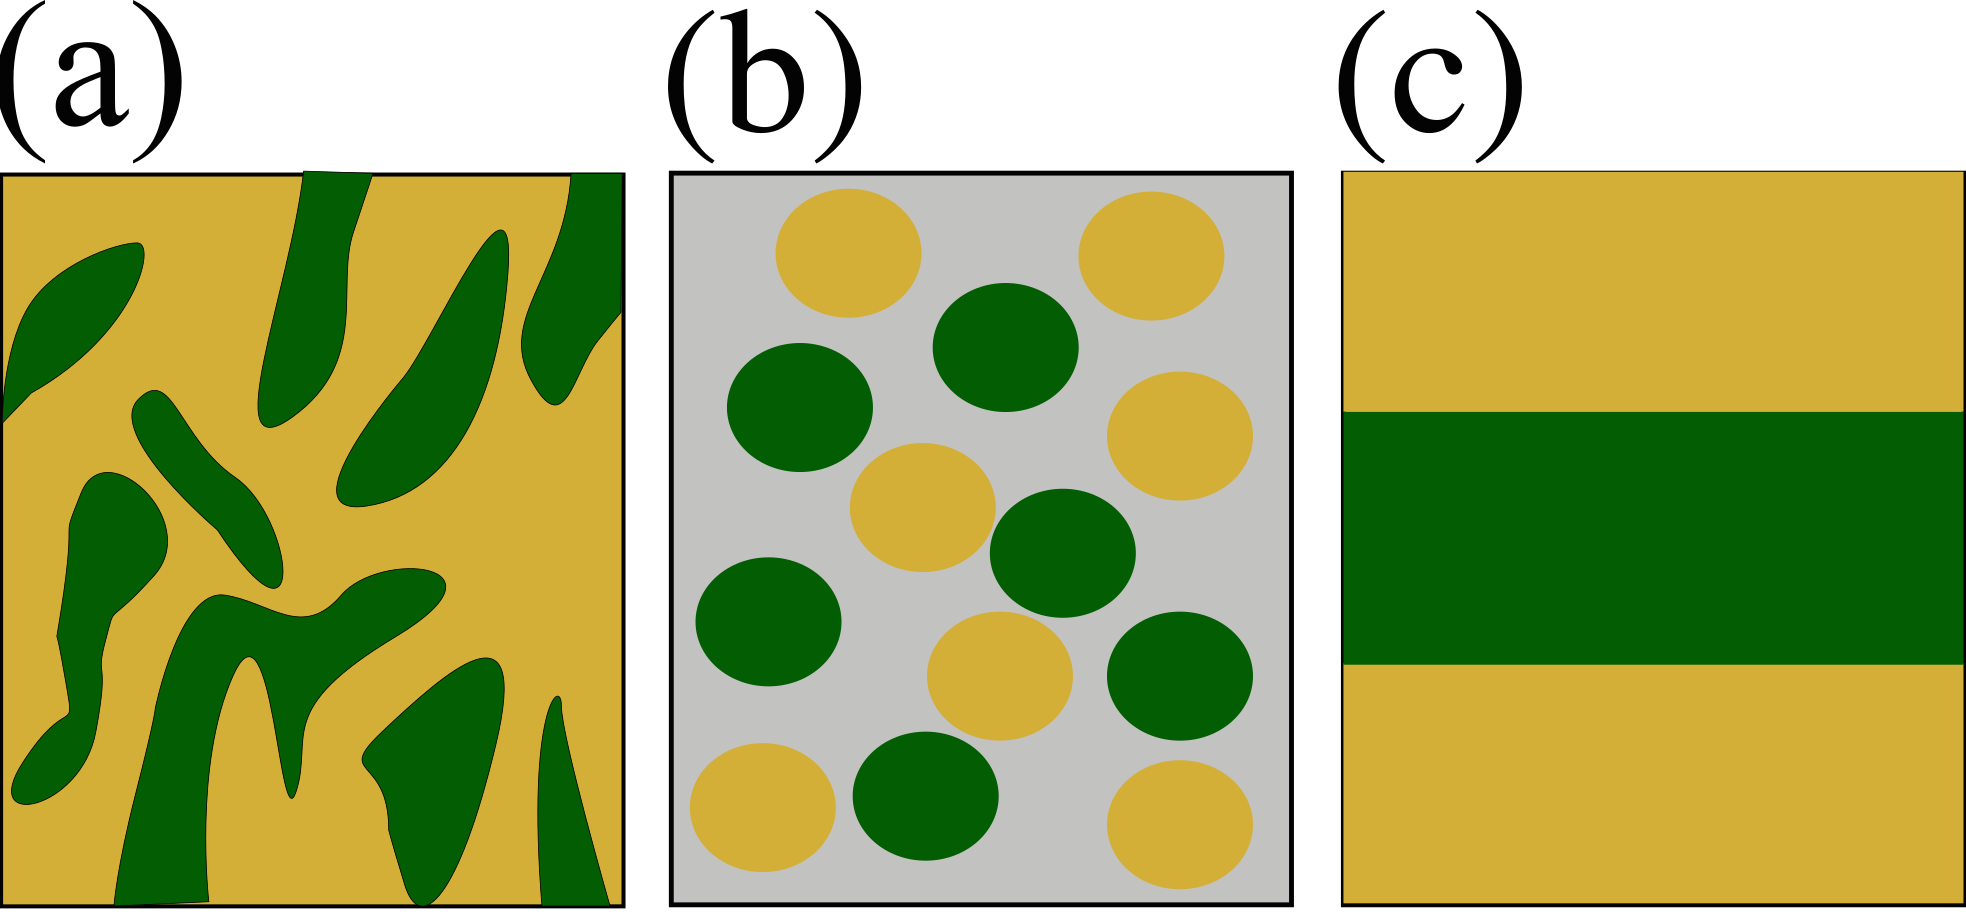
\includegraphics{media/image1.tiff}

Figure . Contours of equal momentum transfer \(\mathbf{k}\) (labeled in
units of Å\textsuperscript{-1}) in energy and scattering angle.
Angle-dispersive x-ray diffraction (AD-XRD) and energy-dispersive x-ray
diffraction (ED-XRD) take vertical and horizontal cuts, respectively, to
achieve broad coverage in \(\mathbf{k}\) and thus obtain information
about the radial distribution function.

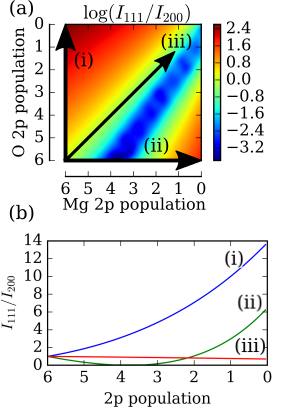
\includegraphics{media/image2.tiff}

Figure . Schematic representations of (a) and (b) angle-dispersive x-ray
diffraction, compared to (c) energy-dispersive x-ray diffraction
(ED-XRD).

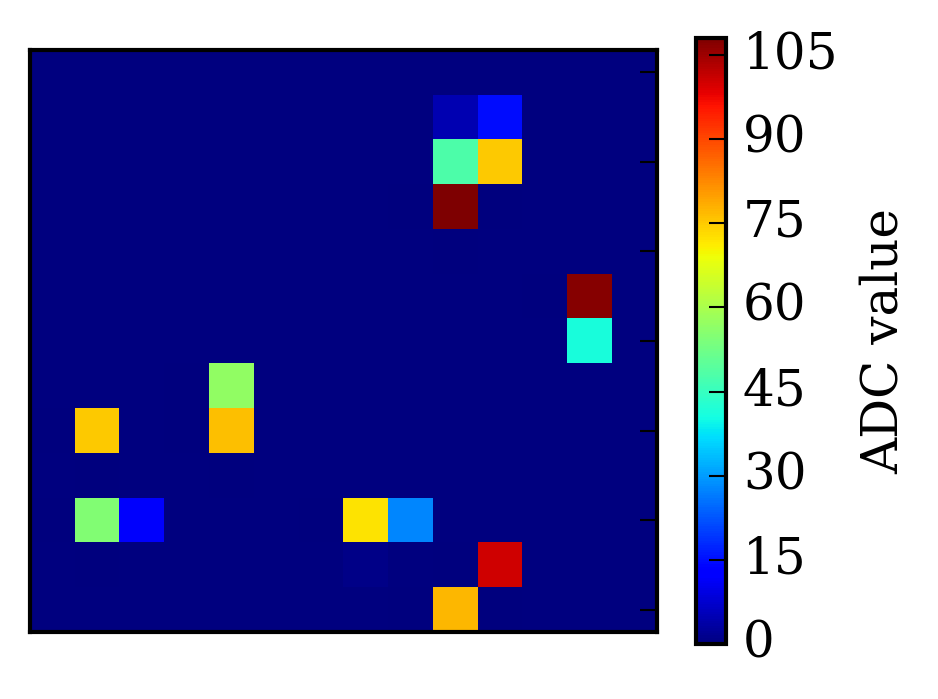
\includegraphics{media/image3.tiff}

\hyperdef{}{ux5fRef350527403}{}{}Figure . Red: experimental thermal
backlighter spectrum from OMEGA
\hyperref[b.-yaakobi-2012-private-communication.]{\textsuperscript{43}}\emph{.}
Blue: a short-pulse Cu \emph{K\textsubscript{α}} backlighter spectrum,
based on scaling of results from a lower energy laser system to a 2.5
kJ, 10 ps laser shot at OMEGA
\hyperref[p.-m.-nilson-2012-private-communication.]{\textsuperscript{44}}\textsuperscript{,}
\hyperref[k.-u.-akli-et-al.-physics-of-plasmas-14-023102-2007.]{\textsuperscript{45}}\hyperref[b.-a.-mattern-g.-t.-seidler-j.-j.-kas-j.-i.-pacold-and-j.-j.-rehr-physical-review-b-85-115135-2012.]{}.

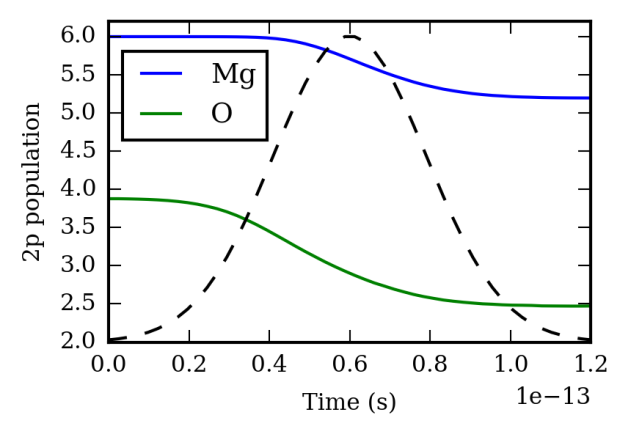
\includegraphics{media/image4.tiff}

Figure . (a): Liquid structure factor of B at 2400K. The original data
(red) of Krishnan \emph{et al.}
\hyperref[s.-krishnan-s.-ansell-j.-j.-felten-k.-j.-volin-and-d.-l.-price-physical-review-letters-81-586-1998.]{\textsuperscript{46}}
contains sharp unphysical noise; we therefore use the filtered
interpolation (blue) of the data for
\(\mathbf{S}\mathbf{(}\mathbf{k}\mathbf{)}\) throughout this paper. (b):
Equivalent theoretical curve for shock-compressed Al at electron density
\(\mathbf{n}_{\mathbf{e}}\) = 5.4 × 10\textsuperscript{23}
cm\textsuperscript{-3} and temperature \(\mathbf{T}_{\mathbf{e}}\) = 10
eV based on Ma \emph{et al.}
\hyperref[t.-ma-et-al.-physical-review-letters-110-065001-2013.]{\textsuperscript{35}}
The curve is based on an approximate treatment of this system's atomic
form factor (see the text for details).

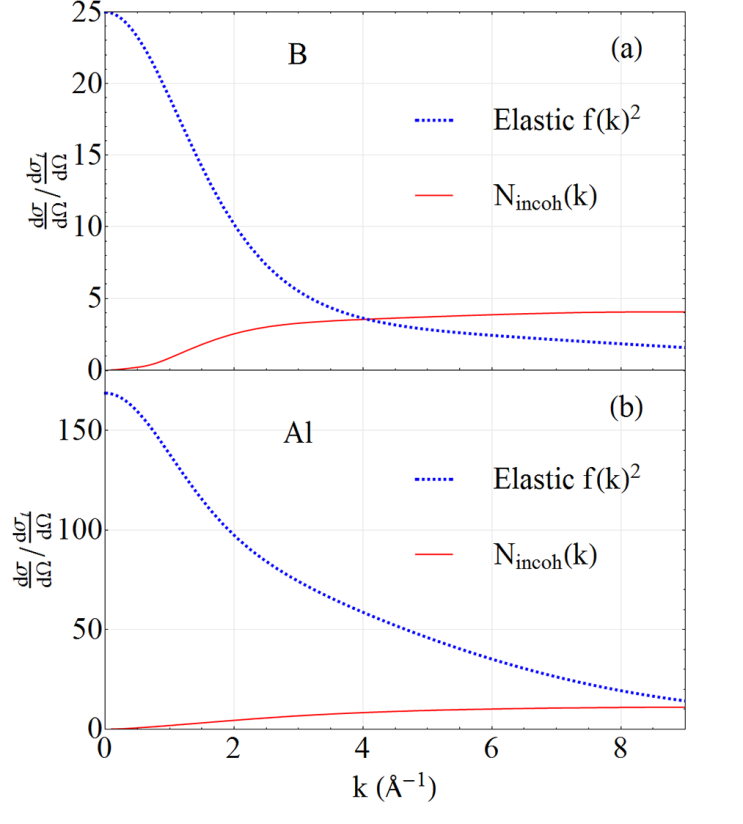
\includegraphics{media/image5.tiff}

Figure . Elastic and inelastic contributions to the differential cross
section of (a) boron and (b) aluminum. The elastic cross sections are
based on tabulated values of \(\mathbf{f(k)}\). The inelastic
differential cross sections, defined by
\(\mathbf{N}_{\mathbf{\text{incoh}}}\left( \mathbf{k} \right)\mathbf{= \ }\int_{\mathbf{0}}^{\mathbf{\infty}}{\mathbf{d}\mathbf{E}^{\mathbf{'}}}\mathbf{\text{\ S}}\left( \mathbf{k,\ }\mathbf{\omega}^{\mathbf{'}} \right)\mathbf{,}\)
are based on
\(\mathbf{S}\left( \mathbf{k,\ }\mathbf{\omega}^{\mathbf{'}} \right)\)
generated from \emph{f}-summed, truncated Compton profiles in the
impulse approximation. See the text for further details.

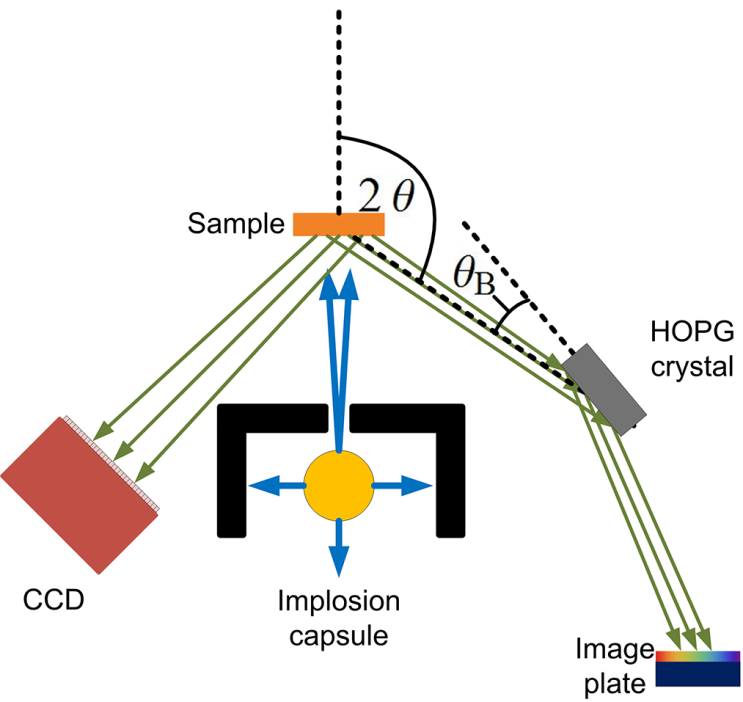
\includegraphics{media/image6.tiff}

\hyperdef{}{ux5fRef350529840}{}{}Figure . Experimental configuration for
ED-XRD at a laser shock facility. A long pulse-driven CH capsule emits a
broad thermal spectrum. Scattering from the target is observed using an
HOPG spectrometer or a CCD in the single-photon hit regime.

\subsection{\texorpdfstring{\protect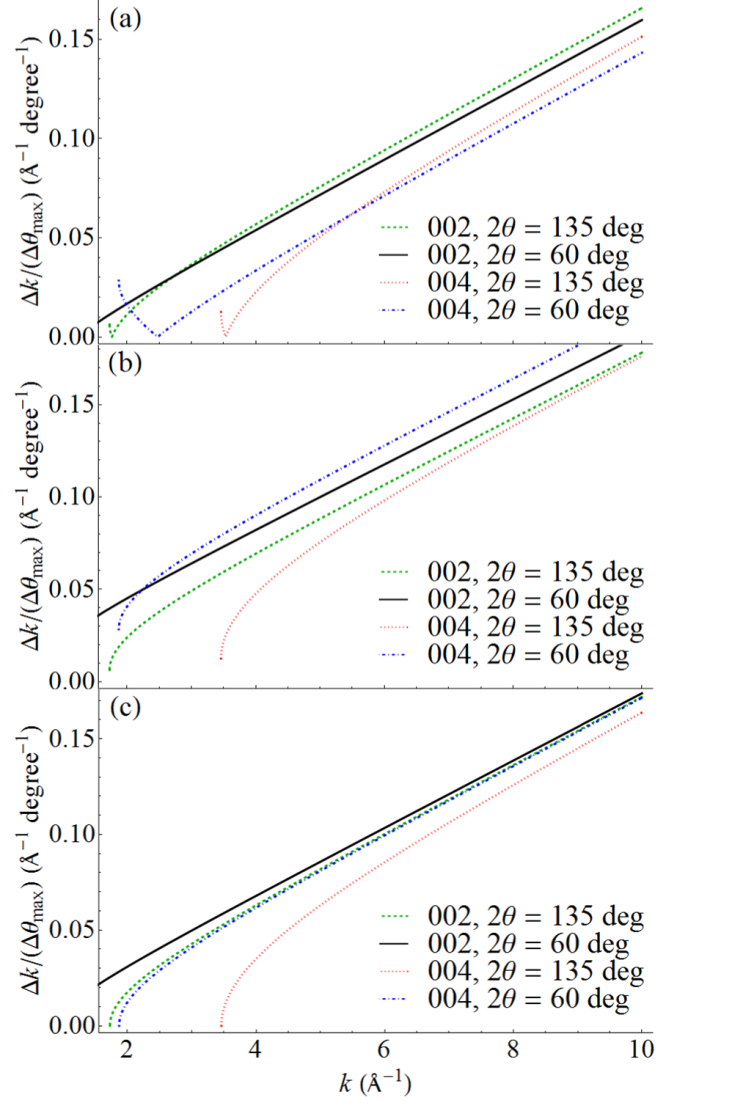
\includegraphics{media/image7.tiff}}{}}\label{section-4}

Figure . Range Δ\emph{k} in momentum transfer of scattering off the
target probed by a small HOPG crystal per degree of its maximum
subtended angle, \(\mathbf{\theta}_{\mathbf{\max}}\), for three
spectrometer geometries that involve the same position (but different
rotations) of the HOPG crystal: (a) the detector located in the target
scattering plane and away from the axis passing through the backlighter
and target, (b) the detector located in the target scattering plane and
near the axis passing through the backlighter and target, and (c) the
detector located such that it, the target, and the HOPG crystal define a
plane perpendicular to the scattering plane. θ\textsubscript{max}
denotes the maximum possible subtended angle of the HOPG crystal given a
fixed spectrometer working distance \(\mathbf{F}\); \emph{i.e.}, for a
crystal of length \(\mathbf{l}\), the maximum subtended angle is
\(\mathbf{\theta}_{\mathbf{\max}}\mathbf{= \ l/F}\)\emph{.}

\hyperdef{}{ux5fRef350527476}{}{}

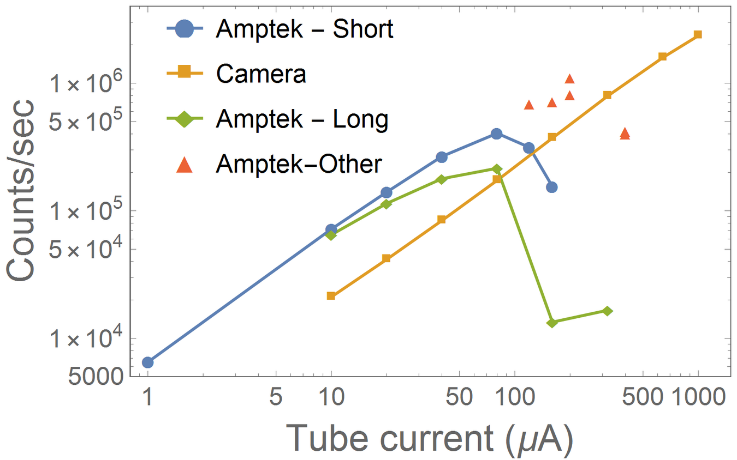
\includegraphics{media/image8.tiff}

Figure . Photon-energy histograms for energy-dispersive diffraction
spectra of liquid boron on CCD and HOPG spectrometers. The expectation
value of photon counts/pixel on the CCD is \(\mathbf{p}\) \emph{=} 0.1.
The energy range of a specific HOPG configuration using a 12-cm long
HOPG analyzer is denoted by the shaded region, the width of which
corresponds to the spectrometer configuration of Fig. 7 (a). The
spectrometer's focal length is 25 cm, and the length of the crystal in
the non-energy dispersive orientation is 12 cm; both spectrometers are
positioned at \(\mathbf{2\theta = 135}\) deg. A 20-µm thick Be foil is
used to reject low-energy photons. Error bars in the HOPG histogram are
smaller than the size of the symbols.

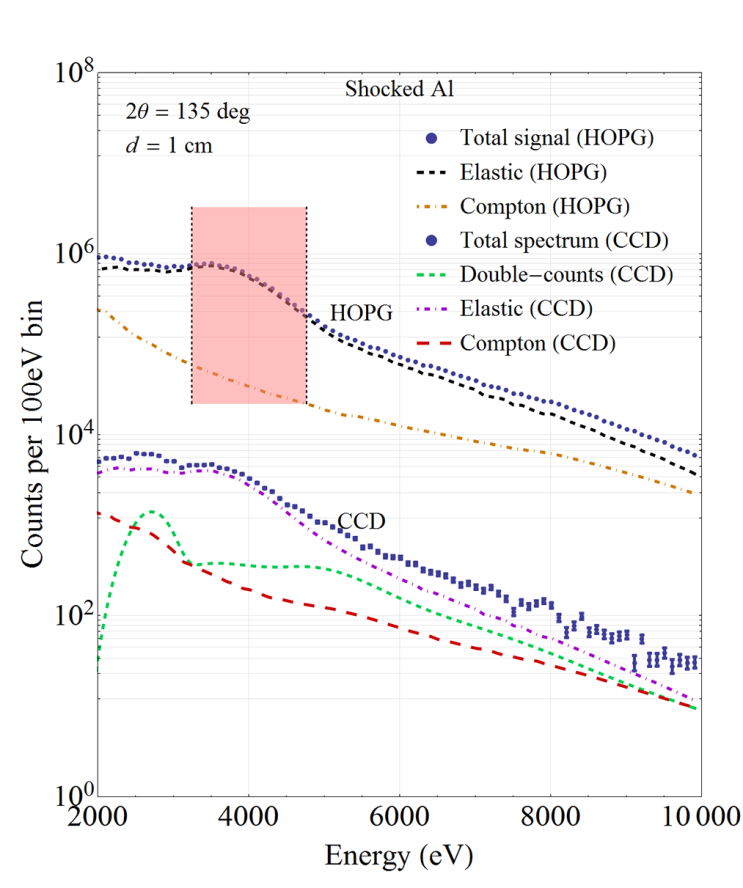
\includegraphics{media/image9.tiff}

\hyperdef{}{ux5fRef350528190}{}{}Figure . Photon-energy histograms on
CCD and HOPG spectrometers for shock-compressed Al at electron density
\(\mathbf{n}_{\mathbf{e}}\) = 5.4 × 10\textsuperscript{23}
cm\textsuperscript{-3} and temperature \(\mathbf{T}_{\mathbf{e}}\) = 10
eV, using Ma \emph{et al.}'s best-fitting theoretical model to their
experimental results for
\({\mathbf{f}\mathbf{(}\mathbf{k}\mathbf{)}}^{\mathbf{2}}\)
\(\mathbf{S}\mathbf{(}\mathbf{k}\mathbf{)}\)
\hyperref[t.-ma-et-al.-physical-review-letters-110-065001-2013.]{\textsuperscript{35}},
and assuming \(\mathbf{f}\mathbf{(}\mathbf{k}\mathbf{)}\) of ambient Al.
The expectation value of photon counts/pixel on the CCD is
\(\mathbf{p}\) \emph{=} 0.1. The energy range of a specific HOPG
configuration using a 12-cm long HOPG analyzer is denoted by the shaded
region, the width of which corresponds to the spectrometer configuration
of Fig. 7 (a). The spectrometer's focal length is 25 cm, and the length
of the crystal in the non-energy dispersive orientation is 12 cm; both
spectrometers are positioned at \(\mathbf{2\theta = 135}\) deg. A 20-µm
thick Be foil is used to reject low-energy photons. Error bars in the
HOPG histogram are smaller than 1\% (not shown).

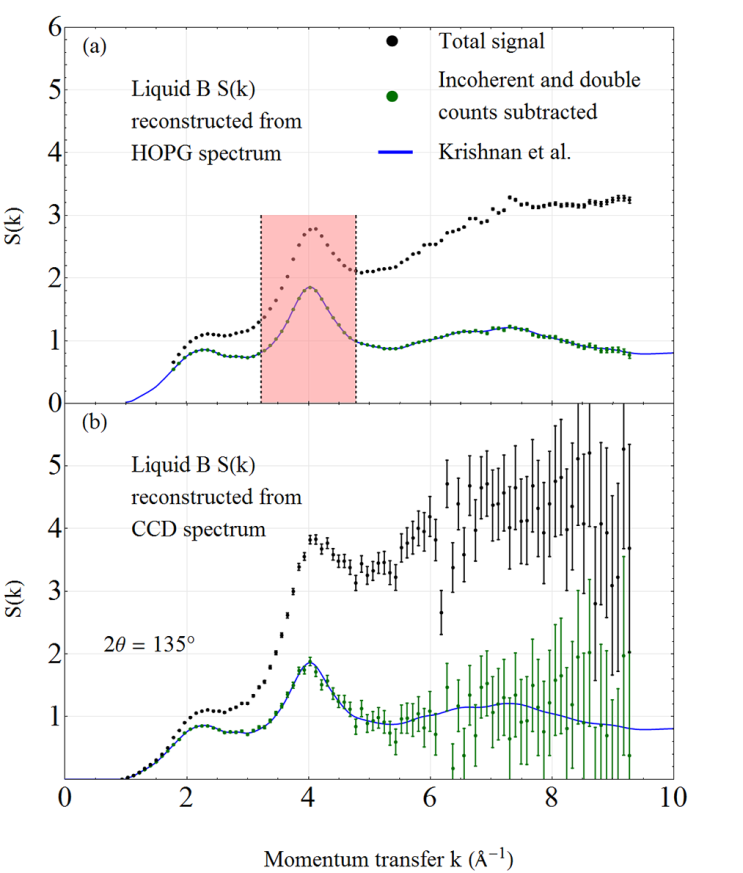
\includegraphics{media/image10.tiff}

\hyperdef{}{ux5fRef350528319}{}{}Figure .
\(\mathbf{S}\mathbf{(}\mathbf{k}\mathbf{)}\) for liquid boron
reconstructed from simulated energy-dispersive spectra of Fig. 8 for (a)
an HOPG spectrometer and (b) a CCD, with and without subtraction of
Compton background and photon double-counts. Data bin size is 100 eV.
The shaded \(\mathbf{k}\)-range in the HOPG spectrum corresponds to the
spectrometer configuration described in the text, and is centered about
the main correlation peak in \(\mathbf{S(k)}\).

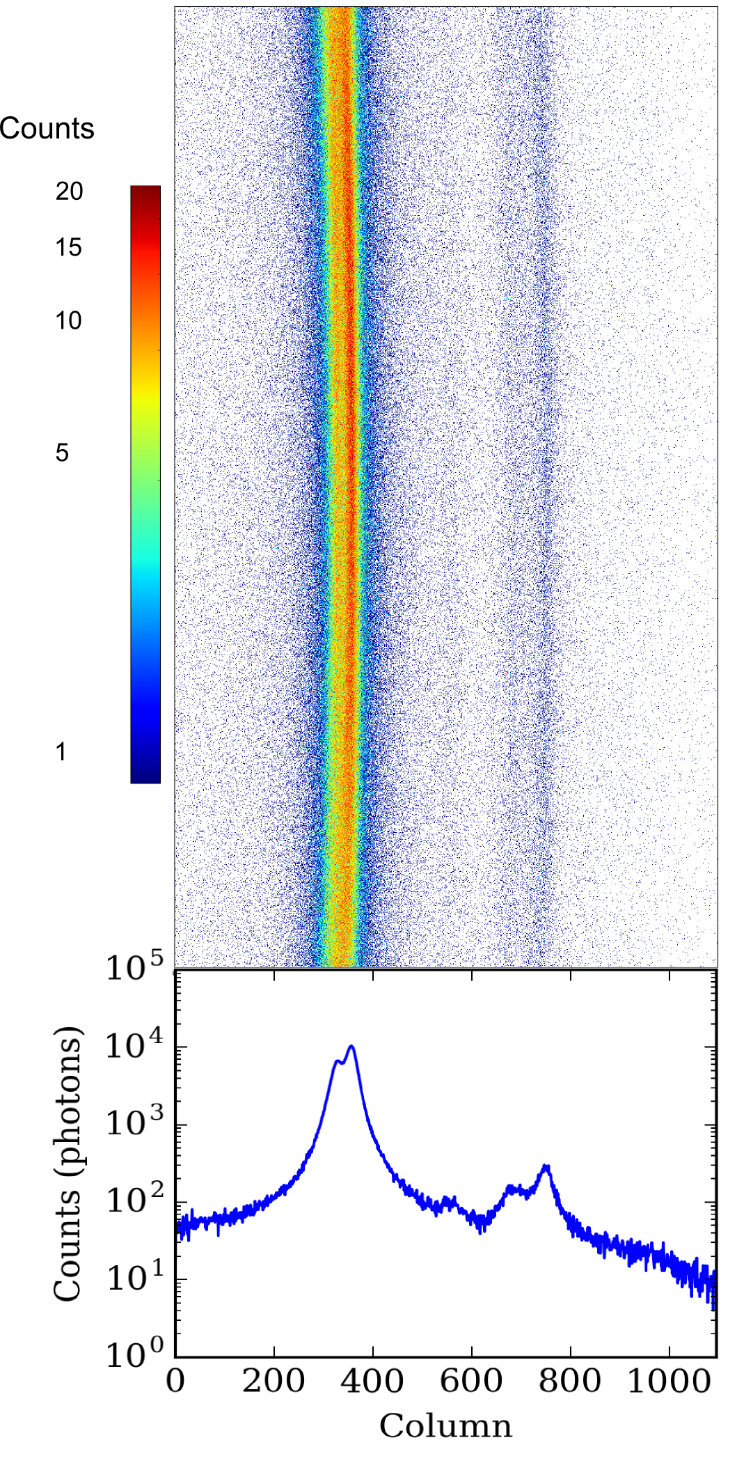
\includegraphics{media/image11.tiff}

\hyperdef{}{ux5fRef350528323}{}{}

Figure . In blue: X-ray structure factor
\(\mathbf{S}\mathbf{(}\mathbf{k}\mathbf{)}\) for shock-compressed Al
computed from Ma, \emph{et al.}
\hyperref[t.-ma-et-al.-physical-review-letters-110-065001-2013.]{\textsuperscript{35}}.
Overlaid with \(\mathbf{S}\mathbf{(}\mathbf{k}\mathbf{)}\) reconstructed
from the spectra of Fig. 9 for (a) an HOPG spectrometer and (b) a CCD.
The data bin size is 100 eV. The shaded \(\mathbf{k}\)-range in the HOPG
spectrum corresponds to the spectrometer configuration described in the
text and is centered about the main correlation peak in
\(\mathbf{S(k)}\).

\subsection{}\label{section-5}

\subsection{}\label{section-6}

\subsection{}\label{section-7}

\subsection{}\label{section-8}

\subsection{}\label{section-9}

\subsection{}\label{section-10}
